\documentclass[11pt, letterpaper]{article}

% Fonts and Encoding
\usepackage[utf8]{inputenc}
\usepackage[T1]{fontenc}
\usepackage{lmodern} % High-quality Latin Modern vector font

% Math and Symbols
\usepackage{amsmath, amssymb, amsthm, amsfonts, mathrsfs, mathtools}

% Layout and Geometry
\usepackage{geometry}
\geometry{letterpaper, margin=1in}
\setlength{\parindent}{0pt}
\setlength{\parskip}{0.6em}

% Formatting and Graphics
\usepackage{graphicx, xcolor, enumitem, booktabs, array, tabularx}

% TikZ for Illustrations
\usepackage{tikz}
\usetikzlibrary{arrows.meta, positioning, shapes.geometric, calc, backgrounds, matrix}

% Clickable Links and TOC
\usepackage{hyperref}
\hypersetup{
    colorlinks=true,
    linkcolor=blue,
    filecolor=magenta,      
    urlcolor=cyan,
    pdftitle={Advanced Mathematics Topic},
}

% Theorem Environments
\newtheorem{theorem}{Theorem}[section]
\newtheorem{lemma}[theorem]{Lemma}
\newtheorem{proposition}[theorem]{Proposition}
\newtheorem{corollary}[theorem]{Corollary}
\theoremstyle{definition}
\newtheorem{definition}{Definition}[section]
\newtheorem{axiom}{Axiom}[section]
\newtheorem{example}{Example}[section]
\theoremstyle{remark}
\newtheorem{remark}{Remark}[section]

% Custom Commands (Enforced standard notation)
\newcommand{\R}{\mathbb{R}}
\newcommand{\N}{\mathbb{N}}
\newcommand{\Z}{\mathbb{Z}}
\newcommand{\Q}{\mathbb{Q}}
\newcommand{\E}{\mathbb{E}}
\newcommand{\Prob}{\mathbb{P}}
\newcommand{\F}{\mathcal{F}}

\title{Section 7.3: Constrained Optimization of Quadratic Forms}
\author{Tashfeen Omran}
\date{\today}

\begin{document}

\maketitle
\tableofcontents
\newpage

% ==============================================================================
% PART 1
% ==============================================================================
\section{Comprehensive Introduction, Context, and Prerequisites}

\subsection{Core Concepts}
In many branches of engineering, economics, physics, and data science, one is required not merely to evaluate a quadratic form $Q(\mathbf{x}) = \mathbf{x}^T A \mathbf{x}$ across all of $\R^n$, but to find its extreme (maximum and minimum) values when $\mathbf{x}$ is restricted to a compact subset of $\R^n$. Without a constraint, a non-zero quadratic form is unbounded: scaling $\mathbf{x}$ by $c > 0$ scales $Q(c\mathbf{x}) = c^2 Q(\mathbf{x})$, sending values toward $+\infty$ or $-\infty$. The canonical constraint restricts $\mathbf{x}$ to the set of \emph{unit vectors} in $\R^n$ (the unit $(n-1)$-sphere $S^{n-1}$).

\begin{definition}[Unit Sphere Constraint]
A vector $\mathbf{x} = (x_1, x_2, \dots, x_n)^T \in \R^n$ satisfies the unit-vector constraint if any of the following four equivalent conditions holds:
\[
\|\mathbf{x}\| = 1, \qquad \|\mathbf{x}\|^2 = 1, \qquad \mathbf{x}^T \mathbf{x} = 1, \qquad x_1^2 + x_2^2 + \cdots + x_n^2 = 1.
\]
\end{definition}

Because $Q(\mathbf{x}) = \mathbf{x}^T A \mathbf{x}$ is a continuous real-valued function defined on the compact (closed and bounded) unit sphere $\{\mathbf{x} \in \R^n : \|\mathbf{x}\| = 1\}$, the Extreme Value Theorem guarantees that $Q$ attains a global minimum $m$ and a global maximum $M$ on this sphere:
\[
m = \min\left\{\mathbf{x}^T A \mathbf{x} : \|\mathbf{x}\| = 1\right\}, \qquad M = \max\left\{\mathbf{x}^T A \mathbf{x} : \|\mathbf{x}\| = 1\right\}.
\]
Here, \emph{minimum} and \emph{maximum} (as well as \emph{least} and \emph{greatest}) refer strictly to the natural ordering of the real numbers ($\R$), not to absolute magnitudes. Moreover, because the unit sphere is path-connected for $n \ge 2$, the Intermediate Value Theorem (verified directly in Exercise~13) implies that the image of the unit sphere under $Q$ is the entire closed interval $[m, M]$.

A central revelation of linear algebra is that when $A$ is a real symmetric $n \times n$ matrix ($A^T = A$), the constrained extrema $M$ and $m$ are precisely the greatest and least eigenvalues of $A$, and the points on the unit sphere where these extrema occur are the corresponding unit eigenvectors. Furthermore, imposing sequential orthogonality constraints $\mathbf{x}^T \mathbf{u}_1 = 0, \dots, \mathbf{x}^T \mathbf{u}_{k-1} = 0$ isolates each intermediate eigenvalue $\lambda_k$ in descending order $\lambda_1 \ge \lambda_2 \ge \cdots \ge \lambda_n$.

\subsection{Intuition and Derivation}
Why do eigenvalues govern the constrained optimization of $\mathbf{x}^T A \mathbf{x}$ on the unit sphere? The answer unfolds in two steps: first analyzing the diagonal case (no cross-product terms), and then reducing the general symmetric case to the diagonal case via an orthogonal change of variable.

\subsubsection*{Step 1: The Diagonal Case}
Suppose $D = \operatorname{diag}(\lambda_1, \lambda_2, \dots, \lambda_n)$ with eigenvalues ordered so that $\lambda_1 \ge \lambda_2 \ge \cdots \ge \lambda_n$. For any unit vector $\mathbf{y} = (y_1, \dots, y_n)^T$ satisfying $y_1^2 + \cdots + y_n^2 = 1$, each $y_i^2 \ge 0$, so replacing every $\lambda_i$ by $\lambda_1$ produces an upper bound, and replacing every $\lambda_i$ by $\lambda_n$ produces a lower bound:
\[
\lambda_n = \lambda_n \sum_{i=1}^n y_i^2 \le \sum_{i=1}^n \lambda_i y_i^2 = \mathbf{y}^T D \mathbf{y} \le \lambda_1 \sum_{i=1}^n y_i^2 = \lambda_1.
\]
Crucially, the upper bound $\lambda_1$ is actually achieved when $\mathbf{y} = \mathbf{e}_1 = (1, 0, \dots, 0)^T$, and the lower bound $\lambda_n$ is achieved when $\mathbf{y} = \mathbf{e}_n = (0, \dots, 0, 1)^T$.

\subsubsection*{Step 2: Reduction of General Symmetric Matrices via Orthogonal Diagonalization}
By the Spectral Theorem for symmetric matrices, any real symmetric $n \times n$ matrix $A$ admits an orthogonal diagonalization $A = P D P^{-1} = P D P^T$, where $D = \operatorname{diag}(\lambda_1, \dots, \lambda_n)$ with $\lambda_1 \ge \lambda_2 \ge \cdots \ge \lambda_n$ and $P = \begin{bmatrix} \mathbf{u}_1 & \mathbf{u}_2 & \cdots & \mathbf{u}_n \end{bmatrix}$ is an orthogonal matrix ($P^T P = I$) whose columns are orthonormal eigenvectors of $A$.

Under the orthogonal change of variable $\mathbf{x} = P\mathbf{y}$ (equivalently $\mathbf{y} = P^T \mathbf{x}$):
\begin{enumerate}[label=(\arabic*)]
    \item \textbf{Preservation of the Quadratic Form:}
    \[
    \mathbf{x}^T A \mathbf{x} = (P\mathbf{y})^T (P D P^T)(P\mathbf{y}) = \mathbf{y}^T (P^T P) D (P^T P) \mathbf{y} = \mathbf{y}^T D \mathbf{y}.
    \]
    \item \textbf{Preservation of the Unit-Sphere Constraint:}
    \[
    \|\mathbf{x}\|^2 = \mathbf{x}^T \mathbf{x} = (P\mathbf{y})^T (P\mathbf{y}) = \mathbf{y}^T (P^T P)\mathbf{y} = \mathbf{y}^T \mathbf{y} = \|\mathbf{y}\|^2.
    \]
    Thus, $\|\mathbf{x}\| = 1$ if and only if $\|\mathbf{y}\| = 1$. Because $P$ is a rigid rotation/reflection of $\R^n$, $\mathbf{x}$ and $\mathbf{y}$ traverse the exact same unit sphere.
    \item \textbf{Mapping the Maximizer Back to $\mathbf{x}$-Space:}
    The maximum of $\mathbf{y}^T D \mathbf{y}$ on $\|\mathbf{y}\|=1$ is $\lambda_1$ at $\mathbf{y} = \mathbf{e}_1$. Transforming back gives
    \[
    \mathbf{x} = P\mathbf{e}_1 = \begin{bmatrix} \mathbf{u}_1 & \mathbf{u}_2 & \cdots & \mathbf{u}_n \end{bmatrix} \begin{bmatrix} 1 \\ 0 \\ \vdots \\ 0 \end{bmatrix} = \mathbf{u}_1.
    \]
\end{enumerate}

\subsubsection*{Step 3: Sequential Orthogonality Constraints}
If we additionally require $\mathbf{x}^T \mathbf{u}_1 = 0, \dots, \mathbf{x}^T \mathbf{u}_{k-1} = 0$, note that since $\mathbf{x} = P\mathbf{y} = \sum_{i=1}^n y_i \mathbf{u}_i$ and the columns $\{\mathbf{u}_i\}$ are orthonormal,
\[
y_i = \mathbf{u}_i^T \mathbf{x} = \mathbf{x}^T \mathbf{u}_i.
\]
Hence the constraints $\mathbf{x}^T \mathbf{u}_1 = \cdots = \mathbf{x}^T \mathbf{u}_{k-1} = 0$ simply force $y_1 = \cdots = y_{k-1} = 0$! On this restricted subspace, $\mathbf{y}^T \mathbf{y} = \sum_{i=k}^n y_i^2 = 1$ and $\mathbf{y}^T D \mathbf{y} = \sum_{i=k}^n \lambda_i y_i^2 \le \lambda_k \sum_{i=k}^n y_i^2 = \lambda_k$, with equality attained at $\mathbf{y} = \mathbf{e}_k$, i.e., $\mathbf{x} = P\mathbf{e}_k = \mathbf{u}_k$.

Geometrically, in $\R^2$, the level curves $Q(\mathbf{x}) = c$ of a positive definite quadratic form are concentric ellipses aligned along the eigenvectors $\mathbf{u}_1$ and $\mathbf{u}_2$. Finding the extrema on the unit circle corresponds to expanding or shrinking these level ellipses until they are tangent to the unit circle $x_1^2 + x_2^2 = 1$; tangency occurs precisely along the principal axes $\pm\mathbf{u}_1$ and $\pm\mathbf{u}_2$, as illustrated below for $Q(\mathbf{x}) = 3x_1^2 + 3x_2^2 + 2x_1x_2$.

\begin{center}
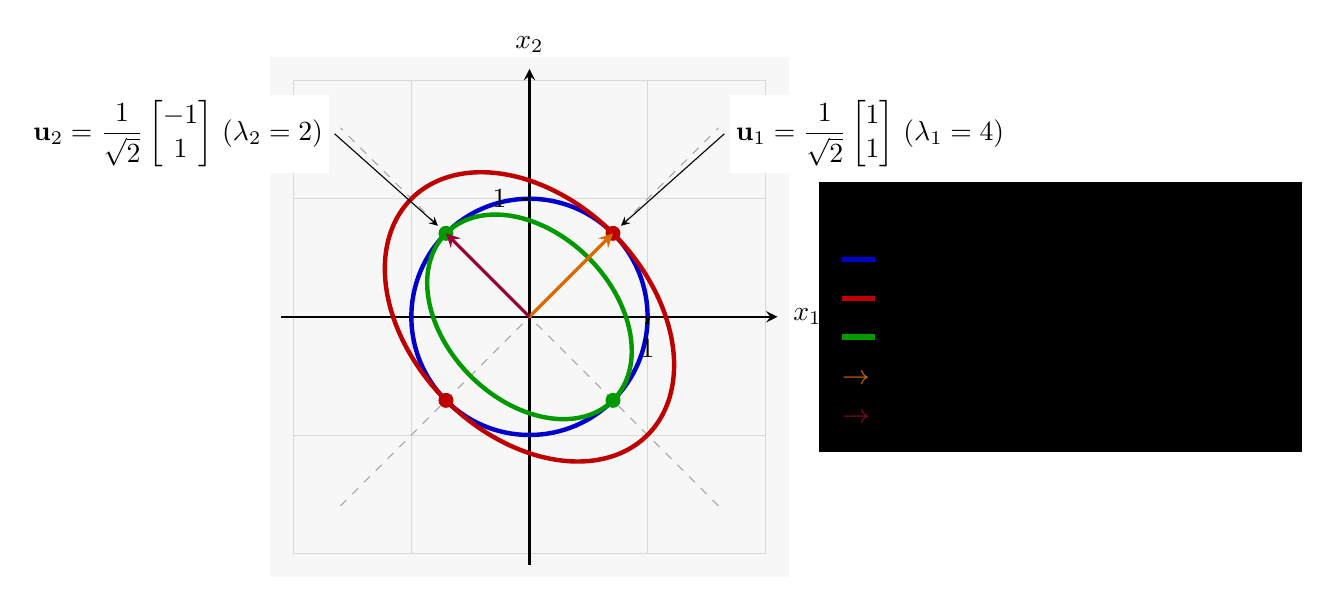
\begin{tikzpicture}[scale=1.5]
    % 1. Background fill
    \fill[gray!6] (-2.2,-2.2) rectangle (2.2,2.2);

    % 2. Grid lines and axes
    \draw[very thin, gray!30] (-2.0,-2.0) grid (2.0,2.0);
    \draw[->, >=stealth, thick] (-2.1,0) -- (2.1,0) node[right=2pt, black] {$x_1$};
    \draw[->, >=stealth, thick] (0,-2.1) -- (0,2.1) node[above=2pt, black] {$x_2$};

    % Principal eigenvector axes (dashed)
    \draw[dashed, gray!70, thin] (-1.6,-1.6) -- (1.6,1.6);
    \draw[dashed, gray!70, thin] (1.6,-1.6) -- (-1.6,1.6);

    % 3. Primary plots
    % Unit circle: x1^2 + x2^2 = 1
    \draw[ultra thick, blue!80!black] (0,0) circle (1);

    % Level curve Q = 4: y1 = 1*cos(t), y2 = sqrt(2)*sin(t) rotated 45 deg
    % x1 = (y1 - y2)/sqrt(2), x2 = (y1 + y2)/sqrt(2)
    \draw[ultra thick, red!75!black, domain=0:360, samples=120, smooth]
        plot ({(1*cos(\x) - 1.4142*sin(\x))/1.4142}, {(1*cos(\x) + 1.4142*sin(\x))/1.4142});

    % Level curve Q = 2: y1 = (1/sqrt(2))*cos(t), y2 = 1*sin(t) rotated 45 deg
    \draw[ultra thick, green!60!black, domain=0:360, samples=120, smooth]
        plot ({(0.7071*cos(\x) - 1*sin(\x))/1.4142}, {(0.7071*cos(\x) + 1*sin(\x))/1.4142});

    % Tangency points
    \fill[red!75!black] (0.7071, 0.7071) circle (1.8pt);
    \fill[red!75!black] (-0.7071, -0.7071) circle (1.8pt);
    \fill[green!60!black] (-0.7071, 0.7071) circle (1.8pt);
    \fill[green!60!black] (0.7071, -0.7071) circle (1.8pt);

    % Unit eigenvectors
    \draw[->, >=stealth, very thick, orange!85!black] (0,0) -- (0.7071, 0.7071);
    \draw[->, >=stealth, very thick, purple!80!black] (0,0) -- (-0.7071, 0.7071);

    % Explicit tick marks on axes
    \draw[thick] (1,0) -- (1,-0.06) node[below=2pt, black] {$1$};
    \draw[thick] (0,1) -- (-0.06,1) node[left=2pt, black] {$1$};

    % 4. Off-axis callouts and single-node legend
    \draw[->, >=stealth, thin, black, shorten >=2pt] (1.65, 1.55) -- (0.74, 0.74);
    \node[right=2pt, align=left, black, fill=white, inner sep=2pt] at (1.65, 1.55) {$\displaystyle \mathbf{u}_1 = \frac{1}{\sqrt{2}}\begin{bmatrix} 1 \\ 1 \end{bmatrix}$ ($\lambda_1 = 4$)};

    \draw[->, >=stealth, thin, black, shorten >=2pt] (-1.65, 1.55) -- (-0.74, 0.74);
    \node[left=2pt, align=right, black, fill=white, inner sep=2pt] at (-1.65, 1.55) {$\displaystyle \mathbf{u}_2 = \frac{1}{\sqrt{2}}\begin{bmatrix} -1 \\ 1 \end{bmatrix}$ ($\lambda_2 = 2$)};

    % Single-node legend anchored in open right margin
    \node[draw, thick, fill=white, align=left, inner sep=8pt, anchor=west, black] at (2.45, 0.0) {
        \textbf{Geometric Legend}\\[4pt]
        \textcolor{blue!80!black}{\rule[0.5ex]{1.2em}{2pt}} Unit Circle: $\mathbf{x}^T\mathbf{x} = 1$\\[2pt]
        \textcolor{red!75!black}{\rule[0.5ex]{1.2em}{2pt}} Outer Tangent: $Q(\mathbf{x}) = 4$ (Max)\\[2pt]
        \textcolor{green!60!black}{\rule[0.5ex]{1.2em}{2pt}} Inner Tangent: $Q(\mathbf{x}) = 2$ (Min)\\[2pt]
        \textcolor{orange!85!black}{\textbf{$\rightarrow$}} Principal Maximizer $\mathbf{u}_1$\\[2pt]
        \textcolor{purple!80!black}{\textbf{$\rightarrow$}} Principal Minimizer $\mathbf{u}_2$
    };
\end{tikzpicture}
\end{center}

\subsection{Historical Context and Motivation}
The constrained optimization of quadratic forms emerged in the eighteenth and nineteenth centuries from two converging pillars of mathematical physics and astronomy: the stability of planetary orbits and the theory of small oscillations in rigid-body mechanics. Leonhard Euler (1758) and Joseph-Louis Lagrange (1788) discovered that finding the principal axes of inertia of a rotating rigid body—directions in which the angular momentum aligns with the angular velocity—is equivalent to finding the extrema of the kinetic-energy quadratic form on the unit sphere. Augustine-Louis Cauchy (1829) subsequently proved that the characteristic roots of a real symmetric matrix are always real, establishing the rigorous algebraic foundation for principal-axis transformations and the Spectral Theorem.

At the turn of the twentieth century, David Hilbert and Erhard Schmidt extended these finite-dimensional variational characterizations to infinite-dimensional integral operators, while Ernst Fischer (1905) and Richard Courant (1920) formulated the general min-max characterization of intermediate eigenvalues. In the modern era, these variational principles became the mathematical backbone of Pearson's Principal Component Analysis (1901) in statistics, Rayleigh–Ritz energy approximations in quantum mechanics, and the Singular Value Decomposition in numerical linear algebra.

\subsection{Key Formulas}
\begin{table}[htbp]
\centering
\renewcommand{\arraystretch}{1.5}
\begin{tabularx}{\textwidth}{>{\raggedright\arraybackslash}p{0.28\textwidth} >{$\displaystyle}l<{$} X}
\toprule
\textbf{Concept} & \text{\textbf{Formula}} & \textbf{Interpretation and Conditions} \\
\midrule
Quadratic Form & Q(\mathbf{x}) = \mathbf{x}^T A \mathbf{x} = \sum_{i=1}^n a_{ii} x_i^2 + 2\sum_{i<j} a_{ij} x_i x_j & $A = [a_{ij}]$ is the unique symmetric $n \times n$ matrix representing $Q$. \\
\addlinespace[4pt]
Unit Constraint & \mathbf{x}^T \mathbf{x} = \|\mathbf{x}\|^2 = \sum_{i=1}^n x_i^2 = 1 & Restricts $\mathbf{x}$ to the compact unit sphere in $\R^n$. \\
\addlinespace[4pt]
Orthogonal Change of Variable & \mathbf{x} = P\mathbf{y}, \quad \mathbf{x}^T A \mathbf{x} = \mathbf{y}^T D \mathbf{y} = \sum_{i=1}^n \lambda_i y_i^2 & $A = P D P^T$ with $P^T P = I$ and $\|\mathbf{x}\| = \|\mathbf{y}\|$. \\
\addlinespace[4pt]
Global Constrained Extrema (Theorem 6) & M = \max_{\|\mathbf{x}\|=1} \mathbf{x}^T A \mathbf{x} = \lambda_1, \quad m = \min_{\|\mathbf{x}\|=1} \mathbf{x}^T A \mathbf{x} = \lambda_n & Eigenvalues ordered $\lambda_1 \ge \lambda_2 \ge \cdots \ge \lambda_n$; attained at unit eigenvectors $\mathbf{u}_1$ and $\mathbf{u}_n$. \\
\addlinespace[4pt]
Second-Order Constrained Max (Theorem 7) & \max_{\substack{\mathbf{x}^T \mathbf{x} = 1 \\ \mathbf{x}^T \mathbf{u}_1 = 0}} \mathbf{x}^T A \mathbf{x} = \lambda_2 & Attained at $\mathbf{x} = \mathbf{u}_2$, a unit eigenvector for $\lambda_2$ orthogonal to $\mathbf{u}_1$. \\
\addlinespace[4pt]
$k$-th Constrained Max (Theorem 8) & \max_{\substack{\mathbf{x}^T \mathbf{x} = 1 \\ \mathbf{x}^T \mathbf{u}_1 = \cdots = \mathbf{x}^T \mathbf{u}_{k-1} = 0}} \mathbf{x}^T A \mathbf{x} = \lambda_k & Attained at $\mathbf{x} = \mathbf{u}_k$ ($k = 2, \dots, n$). \\
\bottomrule
\end{tabularx}
\end{table}

\subsection{Prerequisites}
Mastery of Section~7.3 relies directly on the following foundational skills:
\begin{itemize}
    \item \textbf{Matrix Representation of Quadratic Forms (Section 7.2):} Converting between polynomial expressions $Q(\mathbf{x})$ and symmetric matrices $A$ (putting diagonal coefficients on the diagonal and halving cross-term coefficients onto symmetric off-diagonal entries $a_{ij} = a_{ji} = c_{ij}/2$).
    \item \textbf{Characteristic Polynomials and Eigenvalues (Section 5.2):} Computing $\det(A - \lambda I) = 0$, factoring cubics or quartics (via rational root theorem, row/column symmetries, or block structure), and applying the quadratic formula when roots are irrational.
    \item \textbf{Eigenvectors and Gram–Schmidt Orthogonalization (Sections 5.1, 6.4, 7.1):} Solving $(A - \lambda I)\mathbf{x} = \mathbf{0}$ for bases of eigenspaces, applying Gram–Schmidt if an eigenspace has dimension $\ge 2$, and normalizing vectors via $\mathbf{u} = \mathbf{v}/\|\mathbf{v}\|$.
    \item \textbf{Orthogonal Matrices and Spectral Properties (Section 7.1):} Knowing that eigenvectors of a symmetric matrix corresponding to distinct eigenvalues are automatically orthogonal ($\mathbf{u}_i^T \mathbf{u}_j = 0$), and that orthogonal matrices satisfy $P^{-1} = P^T$ and preserve Euclidean norms ($\|P\mathbf{y}\| = \|\mathbf{y}\|$).
\end{itemize}

% ==============================================================================
% PART 2
% ==============================================================================
\section{Detailed Homework Solutions}

In this section, every exercise from Section~7.3 (Exercises~1 through~17) is solved completely, with the original problem stated verbatim prior to each solution.

% --- Exercise 1 ---
\subsection{Exercise 1}
\textbf{Original Problem:} Find the change of variable $\mathbf{x} = P\mathbf{y}$ that transforms the quadratic form $\mathbf{x}^T A \mathbf{x}$ into $\mathbf{y}^T D \mathbf{y}$ as shown:
\[
5x_1^2 + 4x_2^2 + 3x_3^2 + 4x_1x_2 + 4x_2x_3 = 7y_1^2 + 4y_2^2 + y_3^2.
\]

\textbf{Solution:}
First, construct the symmetric matrix $A$ of the quadratic form $Q(\mathbf{x}) = 5x_1^2 + 4x_2^2 + 3x_3^2 + 4x_1x_2 + 4x_2x_3$. The diagonal entries are the coefficients of $x_1^2, x_2^2, x_3^2$, and each off-diagonal entry $a_{ij} = a_{ji}$ is half the coefficient of $x_i x_j$:
\[
A = \begin{bmatrix} 5 & 2 & 0 \\ 2 & 4 & 2 \\ 0 & 2 & 3 \end{bmatrix}.
\]
From the transformed quadratic form $7y_1^2 + 4y_2^2 + y_3^2$, the diagonal matrix is $D = \operatorname{diag}(7, 4, 1)$, so the eigenvalues of $A$ are $\lambda_1 = 7$, $\lambda_2 = 4$, and $\lambda_3 = 1$ (indeed, $\operatorname{tr}(A) = 5+4+3 = 12 = 7+4+1$). We find a unit eigenvector for each eigenvalue in the exact order listed in $D$.

\textbf{1. Eigenvalue $\lambda_1 = 7$:}
Solve $(A - 7I)\mathbf{x} = \mathbf{0}$:
\[
A - 7I = \begin{bmatrix} -2 & 2 & 0 \\ 2 & -3 & 2 \\ 0 & 2 & -4 \end{bmatrix} \sim \begin{bmatrix} 1 & -1 & 0 \\ 0 & -1 & 2 \\ 0 & 2 & -4 \end{bmatrix} \sim \begin{bmatrix} 1 & 0 & -2 \\ 0 & 1 & -2 \\ 0 & 0 & 0 \end{bmatrix}.
\]
Thus $x_1 = 2x_3$ and $x_2 = 2x_3$. Setting $x_3 = 1$ yields $\mathbf{v}_1 = \begin{bmatrix} 2 \\ 2 \\ 1 \end{bmatrix}$, with $\|\mathbf{v}_1\| = \sqrt{2^2 + 2^2 + 1^2} = \sqrt{9} = 3$. Normalizing gives
\[
\mathbf{u}_1 = \frac{1}{3}\begin{bmatrix} 2 \\ 2 \\ 1 \end{bmatrix} = \begin{bmatrix} 2/3 \\ 2/3 \\ 1/3 \end{bmatrix}.
\]

\textbf{2. Eigenvalue $\lambda_2 = 4$:}
Solve $(A - 4I)\mathbf{x} = \mathbf{0}$:
\[
A - 4I = \begin{bmatrix} 1 & 2 & 0 \\ 2 & 0 & 2 \\ 0 & 2 & -1 \end{bmatrix} \sim \begin{bmatrix} 1 & 2 & 0 \\ 0 & -4 & 2 \\ 0 & 2 & -1 \end{bmatrix} \sim \begin{bmatrix} 1 & 0 & 1 \\ 0 & 1 & -1/2 \\ 0 & 0 & 0 \end{bmatrix}.
\]
Thus $x_1 = -x_3$ and $x_2 = \frac{1}{2}x_3$. Setting $x_3 = 2$ yields $\mathbf{v}_2 = \begin{bmatrix} -2 \\ 1 \\ 2 \end{bmatrix}$, with $\|\mathbf{v}_2\| = \sqrt{(-2)^2 + 1^2 + 2^2} = 3$. Normalizing gives
\[
\mathbf{u}_2 = \frac{1}{3}\begin{bmatrix} -2 \\ 1 \\ 2 \end{bmatrix} = \begin{bmatrix} -2/3 \\ 1/3 \\ 2/3 \end{bmatrix}.
\]

\textbf{3. Eigenvalue $\lambda_3 = 1$:}
Solve $(A - I)\mathbf{x} = \mathbf{0}$:
\[
A - I = \begin{bmatrix} 4 & 2 & 0 \\ 2 & 3 & 2 \\ 0 & 2 & 2 \end{bmatrix} \sim \begin{bmatrix} 2 & 1 & 0 \\ 0 & 2 & 2 \\ 0 & 2 & 2 \end{bmatrix} \sim \begin{bmatrix} 1 & 0 & -1/2 \\ 0 & 1 & 1 \\ 0 & 0 & 0 \end{bmatrix}.
\]
Thus $x_1 = \frac{1}{2}x_3$ and $x_2 = -x_3$. Setting $x_3 = 2$ yields $\mathbf{v}_3 = \begin{bmatrix} 1 \\ -2 \\ 2 \end{bmatrix}$, with $\|\mathbf{v}_3\| = \sqrt{1^2 + (-2)^2 + 2^2} = 3$. Normalizing gives
\[
\mathbf{u}_3 = \frac{1}{3}\begin{bmatrix} 1 \\ -2 \\ 2 \end{bmatrix} = \begin{bmatrix} 1/3 \\ -2/3 \\ 2/3 \end{bmatrix}.
\]

Since the eigenvalues $7, 4, 1$ are distinct and $A$ is symmetric, $\{\mathbf{u}_1, \mathbf{u}_2, \mathbf{u}_3\}$ is automatically an orthonormal set. Assembling $P = \begin{bmatrix} \mathbf{u}_1 & \mathbf{u}_2 & \mathbf{u}_3 \end{bmatrix}$ completes the transformation.

\textbf{Final Answer:} The desired change of variable is $\mathbf{x} = P\mathbf{y}$, where
\[
P = \begin{bmatrix} 2/3 & -2/3 & 1/3 \\ 2/3 & 1/3 & -2/3 \\ 1/3 & 2/3 & 2/3 \end{bmatrix}.
\]
(Note: Any column may be negated without affecting the transformation.)

% --- Exercise 2 ---
\subsection{Exercise 2}
\textbf{Original Problem:} Find the change of variable $\mathbf{x} = P\mathbf{y}$ that transforms the quadratic form $\mathbf{x}^T A \mathbf{x}$ into $\mathbf{y}^T D \mathbf{y}$ as shown:
\[
5x_1^2 + 5x_2^2 + 3x_3^2 + 10x_1x_2 + 4x_1x_3 + 4x_2x_3 = 11y_1^2 + 2y_2^2.
\]
\emph{Hint: $\mathbf{x}$ and $\mathbf{y}$ must have the same number of coordinates, so the quadratic form shown here must have a coefficient of zero for $y_3^2$.}

\textbf{Solution:}
Construct the symmetric matrix $A$ of $Q(\mathbf{x})$:
\[
A = \begin{bmatrix} 5 & 5 & 2 \\ 5 & 5 & 2 \\ 2 & 2 & 3 \end{bmatrix}.
\]
From $\mathbf{y}^T D \mathbf{y} = 11y_1^2 + 2y_2^2 + 0y_3^2$, we have $D = \operatorname{diag}(11, 2, 0)$, so the eigenvalues are $\lambda_1 = 11$, $\lambda_2 = 2$, and $\lambda_3 = 0$.

\textbf{1. Eigenvalue $\lambda_1 = 11$:}
Solve $(A - 11I)\mathbf{x} = \mathbf{0}$:
\[
A - 11I = \begin{bmatrix} -6 & 5 & 2 \\ 5 & -6 & 2 \\ 2 & 2 & -8 \end{bmatrix}.
\]
Subtracting row~2 from row~1 gives $-11x_1 + 11x_2 = 0 \implies x_1 = x_2$. Substituting $x_2 = x_1$ into row~3 gives $4x_1 - 8x_3 = 0 \implies x_1 = 2x_3$. Setting $x_3 = 1$ gives $\mathbf{v}_1 = \begin{bmatrix} 2 \\ 2 \\ 1 \end{bmatrix}$ with $\|\mathbf{v}_1\| = 3$. Normalizing yields
\[
\mathbf{u}_1 = \frac{1}{3}\begin{bmatrix} 2 \\ 2 \\ 1 \end{bmatrix} = \begin{bmatrix} 2/3 \\ 2/3 \\ 1/3 \end{bmatrix}.
\]

\textbf{2. Eigenvalue $\lambda_2 = 2$:}
Solve $(A - 2I)\mathbf{x} = \mathbf{0}$:
\[
A - 2I = \begin{bmatrix} 3 & 5 & 2 \\ 5 & 3 & 2 \\ 2 & 2 & 1 \end{bmatrix}.
\]
Subtracting row~2 from row~1 gives $-2x_1 + 2x_2 = 0 \implies x_1 = x_2$. Substituting into row~3 gives $4x_1 + x_3 = 0 \implies x_3 = -4x_1$. Setting $x_1 = 1$ gives $\mathbf{v}_2 = \begin{bmatrix} 1 \\ 1 \\ -4 \end{bmatrix}$, with $\|\mathbf{v}_2\| = \sqrt{1^2 + 1^2 + (-4)^2} = \sqrt{18} = 3\sqrt{2}$. Normalizing yields
\[
\mathbf{u}_2 = \frac{1}{3\sqrt{2}}\begin{bmatrix} 1 \\ 1 \\ -4 \end{bmatrix} = \begin{bmatrix} 1/(3\sqrt{2}) \\ 1/(3\sqrt{2}) \\ -4/(3\sqrt{2}) \end{bmatrix}.
\]

\textbf{3. Eigenvalue $\lambda_3 = 0$:}
Solve $(A - 0I)\mathbf{x} = A\mathbf{x} = \mathbf{0}$:
\[
A = \begin{bmatrix} 5 & 5 & 2 \\ 5 & 5 & 2 \\ 2 & 2 & 3 \end{bmatrix} \sim \begin{bmatrix} 5 & 5 & 2 \\ 2 & 2 & 3 \\ 0 & 0 & 0 \end{bmatrix} \sim \begin{bmatrix} 1 & 1 & 0 \\ 0 & 0 & 1 \\ 0 & 0 & 0 \end{bmatrix}.
\]
Thus $x_3 = 0$ and $x_1 = -x_2$. Setting $x_2 = -1$ gives $\mathbf{v}_3 = \begin{bmatrix} 1 \\ -1 \\ 0 \end{bmatrix}$, with $\|\mathbf{v}_3\| = \sqrt{2}$. Normalizing yields
\[
\mathbf{u}_3 = \begin{bmatrix} 1/\sqrt{2} \\ -1/\sqrt{2} \\ 0 \end{bmatrix}.
\]

\textbf{Final Answer:} The change of variable is $\mathbf{x} = P\mathbf{y}$, where
\[
P = \begin{bmatrix} 2/3 & 1/(3\sqrt{2}) & 1/\sqrt{2} \\ 2/3 & 1/(3\sqrt{2}) & -1/\sqrt{2} \\ 1/3 & -4/(3\sqrt{2}) & 0 \end{bmatrix}.
\]

% --- Exercise 3 ---
\subsection{Exercise 3}
\textbf{Original Problem:} Find (a) the maximum value of $Q(\mathbf{x})$ subject to the constraint $\mathbf{x}^T \mathbf{x} = 1$, (b) a unit vector $\mathbf{u}$ where this maximum is attained, and (c) the maximum of $Q(\mathbf{x})$ subject to the constraints $\mathbf{x}^T \mathbf{x} = 1$ and $\mathbf{x}^T \mathbf{u} = 0$, for
\[
Q(\mathbf{x}) = 5x_1^2 + 4x_2^2 + 3x_3^2 + 4x_1x_2 + 4x_2x_3 \quad \text{(See Exercise 1.)}
\]

\textbf{Solution:}
From Exercise~1, the symmetric matrix $A$ of $Q(\mathbf{x})$ has eigenvalues $\lambda_1 = 7 > \lambda_2 = 4 > \lambda_3 = 1$, with a unit eigenvector corresponding to $\lambda_1 = 7$ given by $\mathbf{u}_1 = \begin{bmatrix} 2/3 \\ 2/3 \\ 1/3 \end{bmatrix}$.
\begin{enumerate}[label=(\alph*)]
    \item By Theorem~6, the maximum value of $Q(\mathbf{x})$ subject to $\mathbf{x}^T \mathbf{x} = 1$ is the greatest eigenvalue of $A$, which is $\lambda_1 = 7$.
    \item By Theorem~6, this maximum is attained at any unit eigenvector corresponding to $\lambda_1 = 7$, namely $\mathbf{u} = \mathbf{u}_1 = \begin{bmatrix} 2/3 \\ 2/3 \\ 1/3 \end{bmatrix}$ (or $-\mathbf{u}_1$).
    \item By Theorem~7, the maximum value of $Q(\mathbf{x})$ subject to $\mathbf{x}^T \mathbf{x} = 1$ and $\mathbf{x}^T \mathbf{u} = 0$ is the second greatest eigenvalue of $A$, which is $\lambda_2 = 4$ (attained at $\mathbf{u}_2 = \begin{bmatrix} -2/3 \\ 1/3 \\ 2/3 \end{bmatrix}$).
\end{enumerate}

\textbf{Final Answer:} (a) $7$; (b) $\mathbf{u} = \begin{bmatrix} 2/3 \\ 2/3 \\ 1/3 \end{bmatrix}$; (c) $4$.

% --- Exercise 4 ---
\subsection{Exercise 4}
\textbf{Original Problem:} Find (a) the maximum value of $Q(\mathbf{x})$ subject to the constraint $\mathbf{x}^T \mathbf{x} = 1$, (b) a unit vector $\mathbf{u}$ where this maximum is attained, and (c) the maximum of $Q(\mathbf{x})$ subject to the constraints $\mathbf{x}^T \mathbf{x} = 1$ and $\mathbf{x}^T \mathbf{u} = 0$, for
\[
Q(\mathbf{x}) = 5x_1^2 + 5x_2^2 + 3x_3^2 + 10x_1x_2 + 4x_1x_3 + 4x_2x_3 \quad \text{(See Exercise 2.)}
\]

\textbf{Solution:}
From Exercise~2, the symmetric matrix $A$ of $Q(\mathbf{x})$ has eigenvalues $\lambda_1 = 11 > \lambda_2 = 2 > \lambda_3 = 0$, and a unit eigenvector corresponding to $\lambda_1 = 11$ is $\mathbf{u}_1 = \begin{bmatrix} 2/3 \\ 2/3 \\ 1/3 \end{bmatrix}$.
\begin{enumerate}[label=(\alph*)]
    \item By Theorem~6, the constrained maximum on $\mathbf{x}^T \mathbf{x} = 1$ is the greatest eigenvalue $\lambda_1 = 11$.
    \item By Theorem~6, this maximum is attained at $\mathbf{u} = \mathbf{u}_1 = \begin{bmatrix} 2/3 \\ 2/3 \\ 1/3 \end{bmatrix}$.
    \item By Theorem~7, the maximum subject to $\mathbf{x}^T \mathbf{x} = 1$ and $\mathbf{x}^T \mathbf{u} = 0$ is the second greatest eigenvalue $\lambda_2 = 2$.
\end{enumerate}

\textbf{Final Answer:} (a) $11$; (b) $\mathbf{u} = \begin{bmatrix} 2/3 \\ 2/3 \\ 1/3 \end{bmatrix}$; (c) $2$.

% --- Exercise 5 ---
\subsection{Exercise 5}
\textbf{Original Problem:} Find (a) the maximum value of $Q(\mathbf{x})$ subject to the constraint $\mathbf{x}^T \mathbf{x} = 1$, (b) a unit vector $\mathbf{u}$ where this maximum is attained, and (c) the maximum of $Q(\mathbf{x})$ subject to the constraints $\mathbf{x}^T \mathbf{x} = 1$ and $\mathbf{x}^T \mathbf{u} = 0$, for
\[
Q(\mathbf{x}) = x_1^2 + x_2^2 - 12x_1x_2.
\]

\textbf{Solution:}
The symmetric matrix of $Q(\mathbf{x})$ is
\[
A = \begin{bmatrix} 1 & -6 \\ -6 & 1 \end{bmatrix}.
\]
Compute the characteristic equation $\det(A - \lambda I) = 0$:
\[
\det\begin{bmatrix} 1 - \lambda & -6 \\ -6 & 1 - \lambda \end{bmatrix} = (1 - \lambda)^2 - 36 = 0 \implies 1 - \lambda = \pm 6 \implies \lambda_1 = 7, \quad \lambda_2 = -5.
\]
\begin{enumerate}[label=(\alph*)]
    \item By Theorem~6, the maximum value of $Q(\mathbf{x})$ subject to $\mathbf{x}^T \mathbf{x} = 1$ is the greatest eigenvalue $\lambda_1 = 7$.
    \item To find a unit eigenvector for $\lambda_1 = 7$, solve $(A - 7I)\mathbf{x} = \mathbf{0}$:
    \[
    A - 7I = \begin{bmatrix} -6 & -6 \\ -6 & -6 \end{bmatrix} \sim \begin{bmatrix} 1 & 1 \\ 0 & 0 \end{bmatrix} \implies x_1 = -x_2.
    \]
    Setting $x_2 = -1$ gives $\mathbf{v}_1 = \begin{bmatrix} 1 \\ -1 \end{bmatrix}$ with $\|\mathbf{v}_1\| = \sqrt{2}$. Normalizing yields
    \[
    \mathbf{u} = \begin{bmatrix} 1/\sqrt{2} \\ -1/\sqrt{2} \end{bmatrix}.
    \]
    \item By Theorem~7, the maximum subject to $\mathbf{x}^T \mathbf{x} = 1$ and $\mathbf{x}^T \mathbf{u} = 0$ is the second greatest eigenvalue $\lambda_2 = -5$.
\end{enumerate}

\textbf{Final Answer:} (a) $7$; (b) $\mathbf{u} = \begin{bmatrix} 1/\sqrt{2} \\ -1/\sqrt{2} \end{bmatrix}$; (c) $-5$.

% --- Exercise 6 ---
\subsection{Exercise 6}
\textbf{Original Problem:} Find (a) the maximum value of $Q(\mathbf{x})$ subject to the constraint $\mathbf{x}^T \mathbf{x} = 1$, (b) a unit vector $\mathbf{u}$ where this maximum is attained, and (c) the maximum of $Q(\mathbf{x})$ subject to the constraints $\mathbf{x}^T \mathbf{x} = 1$ and $\mathbf{x}^T \mathbf{u} = 0$, for
\[
Q(\mathbf{x}) = 4x_1^2 + 7x_2^2 + 4x_1x_2.
\]

\textbf{Solution:}
The symmetric matrix of $Q(\mathbf{x})$ is
\[
A = \begin{bmatrix} 4 & 2 \\ 2 & 7 \end{bmatrix}.
\]
Compute the characteristic equation:
\[
\det\begin{bmatrix} 4 - \lambda & 2 \\ 2 & 7 - \lambda \end{bmatrix} = (4 - \lambda)(7 - \lambda) - 4 = \lambda^2 - 11\lambda + 24 = (\lambda - 8)(\lambda - 3) = 0.
\]
Thus the eigenvalues are $\lambda_1 = 8$ and $\lambda_2 = 3$.
\begin{enumerate}[label=(\alph*)]
    \item By Theorem~6, the maximum value of $Q(\mathbf{x})$ subject to $\mathbf{x}^T \mathbf{x} = 1$ is $\lambda_1 = 8$.
    \item Solve $(A - 8I)\mathbf{x} = \mathbf{0}$:
    \[
    A - 8I = \begin{bmatrix} -4 & 2 \\ 2 & -1 \end{bmatrix} \sim \begin{bmatrix} 2 & -1 \\ 0 & 0 \end{bmatrix} \implies x_2 = 2x_1.
    \]
    Setting $x_1 = 1$ gives $\mathbf{v}_1 = \begin{bmatrix} 1 \\ 2 \end{bmatrix}$ with $\|\mathbf{v}_1\| = \sqrt{1^2 + 2^2} = \sqrt{5}$. Normalizing gives
    \[
    \mathbf{u} = \begin{bmatrix} 1/\sqrt{5} \\ 2/\sqrt{5} \end{bmatrix}.
    \]
    \item By Theorem~7, the maximum subject to $\mathbf{x}^T \mathbf{x} = 1$ and $\mathbf{x}^T \mathbf{u} = 0$ is $\lambda_2 = 3$.
\end{enumerate}

\textbf{Final Answer:} (a) $8$; (b) $\mathbf{u} = \begin{bmatrix} 1/\sqrt{5} \\ 2/\sqrt{5} \end{bmatrix}$; (c) $3$.

% --- Exercise 7 ---
\subsection{Exercise 7}
\textbf{Original Problem:} Let $Q(\mathbf{x}) = -3x_1^2 - 4x_2^2 + 4x_1x_2 - 4x_2x_3$. Find a unit vector $\mathbf{x}$ in $\R^3$ at which $Q(\mathbf{x})$ is maximized, subject to $\mathbf{x}^T \mathbf{x} = 1$. \emph{[Hint: The eigenvalues of the matrix of the quadratic form $Q$ are $1$, $-2$, and $-6$.]}

\textbf{Solution:}
Write the symmetric matrix $A$ of $Q(\mathbf{x})$:
\[
A = \begin{bmatrix} -3 & 2 & 0 \\ 2 & -4 & -2 \\ 0 & -2 & 0 \end{bmatrix}.
\]
Given the eigenvalues $1, -2, -6$, the greatest eigenvalue is $\lambda_1 = 1$. By Theorem~6, the constrained maximum of $Q(\mathbf{x})$ on $\mathbf{x}^T \mathbf{x} = 1$ is attained at a unit eigenvector corresponding to $\lambda_1 = 1$. Solve $(A - I)\mathbf{x} = \mathbf{0}$:
\[
A - I = \begin{bmatrix} -4 & 2 & 0 \\ 2 & -5 & -2 \\ 0 & -2 & -1 \end{bmatrix}.
\]
Row-reduce the augmented matrix (or work directly with the equations): from row~3, $-2x_2 - x_3 = 0 \implies x_3 = -2x_2$. From row~1, $-4x_1 + 2x_2 = 0 \implies x_2 = 2x_1$. Checking row~2 confirms consistency: $2x_1 - 5(2x_1) - 2(-4x_1) = 2x_1 - 10x_1 + 8x_1 = 0$.

Setting $x_1 = 1$ gives the eigenvector $\mathbf{v}_1 = \begin{bmatrix} 1 \\ 2 \\ -4 \end{bmatrix}$, with Euclidean norm
\[
\|\mathbf{v}_1\| = \sqrt{1^2 + 2^2 + (-4)^2} = \sqrt{1 + 4 + 16} = \sqrt{21}.
\]
Dividing by $\|\mathbf{v}_1\|$ yields the unit eigenvector
\[
\mathbf{x} = \frac{1}{\sqrt{21}} \begin{bmatrix} 1 \\ 2 \\ -4 \end{bmatrix} = \begin{bmatrix} 1/\sqrt{21} \\ 2/\sqrt{21} \\ -4/\sqrt{21} \end{bmatrix}.
\]

\textbf{Final Answer:} A unit vector at which $Q(\mathbf{x})$ is maximized is $\mathbf{x} = \begin{bmatrix} 1/\sqrt{21} \\ 2/\sqrt{21} \\ -4/\sqrt{21} \end{bmatrix}$ (or its negative).

% --- Exercise 8 ---
\subsection{Exercise 8}
\textbf{Original Problem:} Let $Q(\mathbf{x}) = 4x_1^2 + 7x_2^2 + 4x_3^2 - 4x_1x_2 + 8x_1x_3 + 4x_2x_3$. Find a unit vector $\mathbf{x}$ in $\R^3$ at which $Q(\mathbf{x})$ is maximized, subject to $\mathbf{x}^T \mathbf{x} = 1$. \emph{[Hint: The eigenvalues of the matrix of the quadratic form $Q$ are $8$ and $-1$.]}

\textbf{Solution:}
The symmetric matrix $A$ of $Q(\mathbf{x})$ is
\[
A = \begin{bmatrix} 4 & -2 & 4 \\ -2 & 7 & 2 \\ 4 & 2 & 4 \end{bmatrix}.
\]
Notice $\operatorname{tr}(A) = 4 + 7 + 4 = 15 = 8 + 8 + (-1)$, so the greatest eigenvalue $\lambda_1 = 8$ has multiplicity $2$. By Theorem~6, $Q(\mathbf{x})$ is maximized at any unit eigenvector corresponding to $\lambda_1 = 8$. Solve $(A - 8I)\mathbf{x} = \mathbf{0}$:
\[
A - 8I = \begin{bmatrix} -4 & -2 & 4 \\ -2 & -1 & 2 \\ 4 & 2 & -4 \end{bmatrix} \sim \begin{bmatrix} 2 & 1 & -2 \\ 0 & 0 & 0 \\ 0 & 0 & 0 \end{bmatrix}.
\]
The eigenspace for $\lambda_1 = 8$ is the two-dimensional plane $2x_1 + x_2 - 2x_3 = 0$, spanned by $\begin{bmatrix} 1 \\ -2 \\ 0 \end{bmatrix}$ and $\begin{bmatrix} 0 \\ 2 \\ 1 \end{bmatrix}$. Choosing $x_1 = 1$ and $x_3 = 0$ gives $x_2 = -2$, i.e., $\mathbf{v}_1 = \begin{bmatrix} 1 \\ -2 \\ 0 \end{bmatrix}$ with $\|\mathbf{v}_1\| = \sqrt{1^2 + (-2)^2 + 0^2} = \sqrt{5}$. Normalizing gives
\[
\mathbf{x} = \begin{bmatrix} 1/\sqrt{5} \\ -2/\sqrt{5} \\ 0 \end{bmatrix}.
\]
(In fact, any unit vector $\mathbf{x}$ satisfying $2x_1 + x_2 - 2x_3 = 0$, such as $\begin{bmatrix} 0 \\ 2/\sqrt{5} \\ 1/\sqrt{5} \end{bmatrix}$, maximizes $Q(\mathbf{x})$.)

\textbf{Final Answer:} A unit vector at which $Q(\mathbf{x})$ is maximized is $\mathbf{x} = \begin{bmatrix} 1/\sqrt{5} \\ -2/\sqrt{5} \\ 0 \end{bmatrix}$.

% --- Exercise 9 ---
\subsection{Exercise 9}
\textbf{Original Problem:} Find the maximum value of $Q(\mathbf{x}) = 8x_1^2 + 6x_2^2 - 2x_1x_2$ subject to the constraint $x_1^2 + x_2^2 = 1$ (Do not go on to find a vector where the maximum is attained.)

\textbf{Solution:}
The symmetric matrix $A$ of $Q(\mathbf{x})$ is
\[
A = \begin{bmatrix} 8 & -1 \\ -1 & 6 \end{bmatrix}.
\]
Compute the characteristic equation $\det(A - \lambda I) = 0$:
\[
(8 - \lambda)(6 - \lambda) - (-1)(-1) = \lambda^2 - 14\lambda + 48 - 1 = \lambda^2 - 14\lambda + 47 = 0.
\]
Using the quadratic formula:
\[
\lambda = \frac{14 \pm \sqrt{14^2 - 4(1)(47)}}{2} = \frac{14 \pm \sqrt{196 - 188}}{2} = \frac{14 \pm \sqrt{8}}{2} = 7 \pm \sqrt{2}.
\]
By Theorem~6, the maximum value of $Q(\mathbf{x})$ subject to $\mathbf{x}^T \mathbf{x} = x_1^2 + x_2^2 = 1$ is the greatest eigenvalue $\lambda_1 = 7 + \sqrt{2}$.

\textbf{Final Answer:} $7 + \sqrt{2}$.

% --- Exercise 10 ---
\subsection{Exercise 10}
\textbf{Original Problem:} Find the maximum value of $Q(\mathbf{x}) = -5x_1^2 + 7x_2^2 - 2x_1x_2$ subject to the constraint $x_1^2 + x_2^2 = 1$ (Do not go on to find a vector where the maximum is attained.)

\textbf{Solution:}
The symmetric matrix $A$ of $Q(\mathbf{x})$ is
\[
A = \begin{bmatrix} -5 & -1 \\ -1 & 7 \end{bmatrix}.
\]
Compute the characteristic equation $\det(A - \lambda I) = 0$:
\[
(-5 - \lambda)(7 - \lambda) - (-1)(-1) = \lambda^2 - 2\lambda - 35 - 1 = \lambda^2 - 2\lambda - 36 = 0.
\]
Applying the quadratic formula:
\[
\lambda = \frac{2 \pm \sqrt{(-2)^2 - 4(1)(-36)}}{2} = \frac{2 \pm \sqrt{4 + 144}}{2} = \frac{2 \pm \sqrt{148}}{2} = \frac{2 \pm 2\sqrt{37}}{2} = 1 \pm \sqrt{37}.
\]
By Theorem~6, the maximum value of $Q(\mathbf{x})$ subject to $x_1^2 + x_2^2 = 1$ is the greatest eigenvalue $\lambda_1 = 1 + \sqrt{37}$.

\textbf{Final Answer:} $1 + \sqrt{37}$.

% --- Exercise 11 ---
\subsection{Exercise 11}
\textbf{Original Problem:} Suppose $\mathbf{x}$ is a unit eigenvector of a matrix $A$ corresponding to an eigenvalue $3$. What is the value of $\mathbf{x}^T A \mathbf{x}$?

\textbf{Solution:}
Because $\mathbf{x}$ is an eigenvector of $A$ corresponding to the eigenvalue $\lambda = 3$, we have $A\mathbf{x} = 3\mathbf{x}$. Because $\mathbf{x}$ is a unit vector, $\|\mathbf{x}\| = 1$, which implies $\mathbf{x}^T \mathbf{x} = \|\mathbf{x}\|^2 = 1$. Substituting these facts into the quadratic form yields
\[
\mathbf{x}^T A \mathbf{x} = \mathbf{x}^T (3\mathbf{x}) = 3(\mathbf{x}^T \mathbf{x}) = 3(1) = 3.
\]

\textbf{Final Answer:} $3$.

% --- Exercise 12 ---
\subsection{Exercise 12}
\textbf{Original Problem:} Let $\lambda$ be any eigenvalue of a symmetric matrix $A$. Justify the statement made in this section that $m \le \lambda \le M$, where $m$ and $M$ are defined as in (2). \emph{[Hint: Find an $\mathbf{x}$ such that $\lambda = \mathbf{x}^T A \mathbf{x}$.]}

\textbf{Solution:}
By definition of an eigenvalue, there exists a nonzero vector $\mathbf{v} \in \R^n$ such that $A\mathbf{v} = \lambda \mathbf{v}$. Define the normalized vector
\[
\mathbf{x} = \frac{1}{\|\mathbf{v}\|}\mathbf{v}.
\]
Then $\|\mathbf{x}\| = 1$ (so $\mathbf{x}^T \mathbf{x} = 1$), and by linearity of matrix multiplication, $A\mathbf{x} = \lambda \mathbf{x}$. Evaluating the quadratic form at $\mathbf{x}$ gives
\[
\mathbf{x}^T A \mathbf{x} = \mathbf{x}^T (\lambda \mathbf{x}) = \lambda (\mathbf{x}^T \mathbf{x}) = \lambda.
\]
Since $\|\mathbf{x}\| = 1$, the number $\lambda = \mathbf{x}^T A \mathbf{x}$ is an element of the set $S = \{\mathbf{z}^T A \mathbf{z} : \|\mathbf{z}\| = 1\}$. By equation~(2),
\[
m = \min S \qquad \text{and} \qquad M = \max S.
\]
Because every element of $S$ lies between its minimum $m$ and its maximum $M$, it follows immediately that $m \le \lambda \le M$.

\textbf{Final Answer:} Choosing a unit eigenvector $\mathbf{x}$ for $\lambda$ gives $\mathbf{x}^T A \mathbf{x} = \lambda$, placing $\lambda$ in the set $\{\mathbf{z}^T A \mathbf{z} : \|\mathbf{z}\| = 1\}$; hence $m \le \lambda \le M$.

% --- Exercise 13 ---
\subsection{Exercise 13}
\textbf{Original Problem:} Let $A$ be an $n \times n$ symmetric matrix, let $M$ and $m$ denote the maximum and minimum values of the quadratic form $\mathbf{x}^T A \mathbf{x}$, where $\mathbf{x}^T \mathbf{x} = 1$, and denote corresponding unit eigenvectors by $\mathbf{u}_1$ and $\mathbf{u}_n$. The following calculations show that given any number $t$ between $M$ and $m$, there is a unit vector $\mathbf{x}$ such that $t = \mathbf{x}^T A \mathbf{x}$. Verify that $t = (1 - \alpha)m + \alpha M$ for some number $\alpha$ between $0$ and $1$. Then let $\mathbf{x} = \sqrt{1 - \alpha}\,\mathbf{u}_n + \sqrt{\alpha}\,\mathbf{u}_1$, and show that $\mathbf{x}^T \mathbf{x} = 1$ and $\mathbf{x}^T A \mathbf{x} = t$.

\textbf{Solution:}
\textbf{Step 1: Existence of $\alpha \in [0, 1]$ such that $t = (1 - \alpha)m + \alpha M$.}
Suppose $m \le t \le M$.
\begin{itemize}
    \item If $M = m$, then $t = m = M$, and any $\alpha \in [0, 1]$ (for example, $\alpha = 1$) satisfies $(1 - \alpha)m + \alpha M = m = t$.
    \item If $M > m$, define
    \[
    \alpha = \frac{t - m}{M - m}.
    \]
    Since $m \le t \le M$ and $M - m > 0$, we have $0 \le t - m \le M - m$, so dividing by $M - m$ yields $0 \le \alpha \le 1$. Moreover,
    \[
    (1 - \alpha)m + \alpha M = m + \alpha(M - m) = m + \frac{t - m}{M - m}(M - m) = m + (t - m) = t.
    \]
\end{itemize}

\textbf{Step 2: Showing $\mathbf{x}^T \mathbf{x} = 1$ and $\mathbf{x}^T A \mathbf{x} = t$.}
If $M = m$, choosing $\alpha = 1$ gives $\mathbf{x} = \mathbf{u}_1$, which trivially satisfies $\mathbf{x}^T\mathbf{x} = 1$ and $\mathbf{x}^T A \mathbf{x} = M = t$. (If $n \ge 2$ and $\mathbf{u}_1, \mathbf{u}_n$ are chosen from an orthonormal eigenbasis, $\mathbf{u}_1^T\mathbf{u}_n = 0$ even when $M = m$.)

For the main case $M > m$, because $A$ is symmetric and $\mathbf{u}_1$ and $\mathbf{u}_n$ correspond to distinct eigenvalues $M$ and $m$, they are orthogonal: $\mathbf{u}_1^T \mathbf{u}_n = \mathbf{u}_n^T \mathbf{u}_1 = 0$. Also, since they are unit eigenvectors, $\mathbf{u}_1^T \mathbf{u}_1 = 1$, $\mathbf{u}_n^T \mathbf{u}_n = 1$, $A\mathbf{u}_1 = M\mathbf{u}_1$, and $A\mathbf{u}_n = m\mathbf{u}_n$. Let $\mathbf{x} = \sqrt{1 - \alpha}\,\mathbf{u}_n + \sqrt{\alpha}\,\mathbf{u}_1$. First, compute $\mathbf{x}^T \mathbf{x}$:
\begin{align*}
\mathbf{x}^T \mathbf{x} &= \left(\sqrt{1 - \alpha}\,\mathbf{u}_n + \sqrt{\alpha}\,\mathbf{u}_1\right)^T \left(\sqrt{1 - \alpha}\,\mathbf{u}_n + \sqrt{\alpha}\,\mathbf{u}_1\right) \\
&= (1 - \alpha)(\mathbf{u}_n^T \mathbf{u}_n) + \sqrt{(1 - \alpha)\alpha}\,(\mathbf{u}_n^T \mathbf{u}_1 + \mathbf{u}_1^T \mathbf{u}_n) + \alpha(\mathbf{u}_1^T \mathbf{u}_1) \\
&= (1 - \alpha)(1) + \sqrt{(1 - \alpha)\alpha}\,(0 + 0) + \alpha(1) \\
&= 1 - \alpha + \alpha = 1.
\end{align*}
Next, compute $A\mathbf{x} = \sqrt{1 - \alpha}\,A\mathbf{u}_n + \sqrt{\alpha}\,A\mathbf{u}_1 = m\sqrt{1 - \alpha}\,\mathbf{u}_n + M\sqrt{\alpha}\,\mathbf{u}_1$, and hence:
\begin{align*}
\mathbf{x}^T A \mathbf{x} &= \left(\sqrt{1 - \alpha}\,\mathbf{u}_n + \sqrt{\alpha}\,\mathbf{u}_1\right)^T \left(m\sqrt{1 - \alpha}\,\mathbf{u}_n + M\sqrt{\alpha}\,\mathbf{u}_1\right) \\
&= (1 - \alpha)m(\mathbf{u}_n^T \mathbf{u}_n) + \sqrt{(1 - \alpha)\alpha}\,(M\,\mathbf{u}_n^T \mathbf{u}_1 + m\,\mathbf{u}_1^T \mathbf{u}_n) + \alpha M(\mathbf{u}_1^T \mathbf{u}_1) \\
&= (1 - \alpha)m(1) + \sqrt{(1 - \alpha)\alpha}\,(0 + 0) + \alpha M(1) \\
&= (1 - \alpha)m + \alpha M = t.
\end{align*}

\textbf{Final Answer:} Setting $\alpha = (t - m)/(M - m) \in [0,1]$ (for $M > m$, and $\alpha=1$ if $M=m$) gives $t = (1-\alpha)m + \alpha M$, and orthogonality $\mathbf{u}_1^T \mathbf{u}_n = 0$ guarantees $\mathbf{x}^T \mathbf{x} = 1$ and $\mathbf{x}^T A \mathbf{x} = t$.

% --- Exercise 14 ---
\subsection{Exercise 14}
\textbf{Original Problem:} Follow the instructions given for Exercises 3–6 for
\[
Q(\mathbf{x}) = 3x_1x_2 + 5x_1x_3 + 7x_1x_4 + 7x_2x_3 + 5x_2x_4 + 3x_3x_4.
\]

\textbf{Solution:}
Construct the symmetric matrix $A$ by halving each cross-term coefficient:
\[
A = \frac{1}{2} \begin{bmatrix} 0 & 3 & 5 & 7 \\ 3 & 0 & 7 & 5 \\ 5 & 7 & 0 & 3 \\ 7 & 5 & 3 & 0 \end{bmatrix}.
\]
Notice that $A$ is bisymmetric (each row is a permutation of the same entries $\{0, 3/2, 5/2, 7/2\}$ reflecting a Klein four-group symmetry). Consequently, the four mutually orthogonal Walsh–Hadamard vectors are exact eigenvectors of $A$:
\begin{enumerate}[label=(\arabic*)]
    \item $\mathbf{v}_1 = \begin{bmatrix} 1 \\ 1 \\ 1 \\ 1 \end{bmatrix}$: \quad $A\mathbf{v}_1 = \frac{1}{2}\begin{bmatrix} 3+5+7 \\ 3+7+5 \\ 5+7+3 \\ 7+5+3 \end{bmatrix} = \frac{15}{2}\mathbf{v}_1 \implies \lambda_1 = \frac{15}{2} = 7.5$.
    \item $\mathbf{v}_2 = \begin{bmatrix} 1 \\ -1 \\ -1 \\ 1 \end{bmatrix}$: \quad $A\mathbf{v}_2 = \frac{1}{2}\begin{bmatrix} -3-5+7 \\ 3-7+5 \\ 5-7+3 \\ 7-5-3 \end{bmatrix} = \frac{1}{2}\begin{bmatrix} -1 \\ 1 \\ 1 \\ -1 \end{bmatrix} = -\frac{1}{2}\mathbf{v}_2 \implies \lambda_2 = -\frac{1}{2} = -0.5$.
    \item $\mathbf{v}_3 = \begin{bmatrix} 1 \\ -1 \\ 1 \\ -1 \end{bmatrix}$: \quad $A\mathbf{v}_3 = \frac{1}{2}\begin{bmatrix} -3+5-7 \\ 3+7-5 \\ 5-7-3 \\ 7-5+3 \end{bmatrix} = \frac{1}{2}\begin{bmatrix} -5 \\ 5 \\ -5 \\ 5 \end{bmatrix} = -\frac{5}{2}\mathbf{v}_3 \implies \lambda_3 = -\frac{5}{2} = -2.5$.
    \item $\mathbf{v}_4 = \begin{bmatrix} 1 \\ 1 \\ -1 \\ -1 \end{bmatrix}$: \quad $A\mathbf{v}_4 = \frac{1}{2}\begin{bmatrix} 3-5-7 \\ 3-7-5 \\ 5+7-3 \\ 7+5-3 \end{bmatrix} = \frac{1}{2}\begin{bmatrix} -9 \\ -9 \\ 9 \\ 9 \end{bmatrix} = -\frac{9}{2}\mathbf{v}_4 \implies \lambda_4 = -\frac{9}{2} = -4.5$.
\end{enumerate}
Verification: $\sum_{i=1}^4 \lambda_i = \frac{15 - 1 - 5 - 9}{2} = 0 = \operatorname{tr}(A)$. The eigenvalues in descending order are $\frac{15}{2} > -\frac{1}{2} > -\frac{5}{2} > -\frac{9}{2}$.
\begin{enumerate}[label=(\alph*)]
    \item By Theorem~6, the maximum value of $Q(\mathbf{x})$ subject to $\mathbf{x}^T \mathbf{x} = 1$ is $\lambda_1 = \frac{15}{2}$ (or $7.5$).
    \item Normalizing $\mathbf{v}_1$ (since $\|\mathbf{v}_1\| = \sqrt{1+1+1+1} = 2$) gives the unit maximizer
    \[
    \mathbf{u} = \frac{1}{2}\begin{bmatrix} 1 \\ 1 \\ 1 \\ 1 \end{bmatrix} = \begin{bmatrix} 1/2 \\ 1/2 \\ 1/2 \\ 1/2 \end{bmatrix}.
    \]
    \item By Theorem~7, the maximum subject to $\mathbf{x}^T \mathbf{x} = 1$ and $\mathbf{x}^T \mathbf{u} = 0$ is the second greatest eigenvalue $\lambda_2 = -\frac{1}{2}$ (or $-0.5$).
\end{enumerate}

\textbf{Final Answer:} (a) $15/2$; (b) $\mathbf{u} = \begin{bmatrix} 1/2 \\ 1/2 \\ 1/2 \\ 1/2 \end{bmatrix}$; (c) $-1/2$.

% --- Exercise 15 ---
\subsection{Exercise 15}
\textbf{Original Problem:} Follow the instructions given for Exercises 3–6 for
\[
Q(\mathbf{x}) = 4x_1^2 - 6x_1x_2 - 10x_1x_3 - 10x_1x_4 - 6x_2x_3 - 6x_2x_4 - 2x_3x_4.
\]

\textbf{Solution:}
Write the symmetric matrix $A$ of $Q(\mathbf{x})$:
\[
A = \begin{bmatrix} 4 & -3 & -5 & -5 \\ -3 & 0 & -3 & -3 \\ -5 & -3 & 0 & -1 \\ -5 & -3 & -1 & 0 \end{bmatrix}.
\]
Notice the symmetry in the last two coordinates ($x_3$ and $x_4$). Immediately, $\mathbf{w} = \begin{bmatrix} 0 \\ 0 \\ 1 \\ -1 \end{bmatrix}$ satisfies
\[
A\mathbf{w} = \begin{bmatrix} 0 \\ 0 \\ 1 \\ -1 \end{bmatrix} = 1\cdot\mathbf{w},
\]
so $\lambda = 1$ is an eigenvalue. The remaining three orthogonal eigenvectors must be orthogonal to $\mathbf{w}$, meaning they have the form $\mathbf{v} = \begin{bmatrix} a \\ b \\ c \\ c \end{bmatrix}$. Applying $A$ to $\mathbf{v}$ gives
\[
A\begin{bmatrix} a \\ b \\ c \\ c \end{bmatrix} = \begin{bmatrix} 4a - 3b - 10c \\ -3a - 6c \\ -5a - 3b - c \\ -5a - 3b - c \end{bmatrix}.
\]
Thus $A\mathbf{v} = \lambda \mathbf{v}$ reduces to the $3 \times 3$ eigenvalue problem $M\begin{bmatrix} a \\ b \\ c \end{bmatrix} = \lambda \begin{bmatrix} a \\ b \\ c \end{bmatrix}$, where $M = \begin{bmatrix} 4 & -3 & -10 \\ -3 & 0 & -6 \\ -5 & -3 & -1 \end{bmatrix}$. Computing $\det(M - \lambda I) = 0$:
\begin{align*}
\det\begin{bmatrix} 4-\lambda & -3 & -10 \\ -3 & -\lambda & -6 \\ -5 & -3 & -1-\lambda \end{bmatrix} &= (4-\lambda)\bigl(\lambda(1+\lambda) - 18\bigr) + 3\bigl(3(1+\lambda) - 30\bigr) - 10(9 - 5\lambda) \\
&= (4-\lambda)(\lambda^2 + \lambda - 18) + (9\lambda - 81) + (50\lambda - 90) \\
&= -\lambda^3 + 3\lambda^2 + 22\lambda - 72 + 59\lambda - 171 \\
&= -\lambda^3 + 3\lambda^2 + 81\lambda - 243 \\
&= -(\lambda - 3)(\lambda^2 - 81) = -(\lambda - 3)(\lambda - 9)(\lambda + 9) = 0.
\end{align*}
Hence the four eigenvalues of $A$ in descending order are $\lambda_1 = 9 > \lambda_2 = 3 > \lambda_3 = 1 > \lambda_4 = -9$. (Check: $\operatorname{tr}(A) = 4 = 9 + 3 + 1 - 9$.)

\begin{enumerate}[label=(\alph*)]
    \item By Theorem~6, the maximum value of $Q(\mathbf{x})$ subject to $\mathbf{x}^T \mathbf{x} = 1$ is $\lambda_1 = 9$.
    \item To find a unit eigenvector for $\lambda_1 = 9$, solve $(M - 9I)\begin{bmatrix} a \\ b \\ c \end{bmatrix} = \mathbf{0}$:
    \[
    \begin{bmatrix} -5 & -3 & -10 \\ -3 & -9 & -6 \\ -5 & -3 & -10 \end{bmatrix} \begin{bmatrix} a \\ b \\ c \end{bmatrix} = \mathbf{0}.
    \]
    Row~2 gives $a + 3b + 2c = 0$, and row~1 gives $5a + 3b + 10c = 0$. Subtracting yields $4a + 8c = 0 \implies a = -2c$, and substituting back yields $3b = 0 \implies b = 0$. Setting $c = -1$ gives $\mathbf{v}_1 = \begin{bmatrix} 2 \\ 0 \\ -1 \\ -1 \end{bmatrix}$ with $\|\mathbf{v}_1\| = \sqrt{2^2 + 0^2 + (-1)^2 + (-1)^2} = \sqrt{6}$. Normalizing gives
    \[
    \mathbf{u} = \frac{1}{\sqrt{6}}\begin{bmatrix} 2 \\ 0 \\ -1 \\ -1 \end{bmatrix}.
    \]
    \item By Theorem~7, the maximum subject to $\mathbf{x}^T \mathbf{x} = 1$ and $\mathbf{x}^T \mathbf{u} = 0$ is the second greatest eigenvalue $\lambda_2 = 3$.
\end{enumerate}

\textbf{Final Answer:} (a) $9$; (b) $\mathbf{u} = \begin{bmatrix} 2/\sqrt{6} \\ 0 \\ -1/\sqrt{6} \\ -1/\sqrt{6} \end{bmatrix}$; (c) $3$.

% --- Exercise 16 ---
\subsection{Exercise 16}
\textbf{Original Problem:} Follow the instructions given for Exercises 3–6 for
\[
Q(\mathbf{x}) = -6x_1^2 - 10x_2^2 - 13x_3^2 - 13x_4^2 - 4x_1x_2 - 4x_1x_3 - 4x_1x_4 + 6x_3x_4.
\]

\textbf{Solution:}
Write the symmetric matrix $A$ of $Q(\mathbf{x})$:
\[
A = \begin{bmatrix} -6 & -2 & -2 & -2 \\ -2 & -10 & 0 & 0 \\ -2 & 0 & -13 & 3 \\ -2 & 0 & 3 & -13 \end{bmatrix}.
\]
Exploit the symmetry of the last three coordinates:
\begin{enumerate}[label=(\arabic*)]
    \item Testing $\mathbf{w}_1 = \begin{bmatrix} 0 \\ 0 \\ 1 \\ -1 \end{bmatrix}$ yields $A\mathbf{w}_1 = \begin{bmatrix} 0 \\ 0 \\ -16 \\ 16 \end{bmatrix} = -16\mathbf{w}_1$, so $\lambda = -16$ is an eigenvalue.
    \item Vectors orthogonal to $\mathbf{w}_1$ have $x_3 = x_4$. Testing $\mathbf{w}_2 = \begin{bmatrix} 0 \\ -2 \\ 1 \\ 1 \end{bmatrix}$ yields $A\mathbf{w}_2 = \begin{bmatrix} 0 \\ 20 \\ -10 \\ -10 \end{bmatrix} = -10\mathbf{w}_2$, so $\lambda = -10$ is an eigenvalue.
    \item Vectors orthogonal to both $\mathbf{w}_1$ and $\mathbf{w}_2$ have the form $\mathbf{v} = \begin{bmatrix} a \\ b \\ b \\ b \end{bmatrix}$. Applying $A$ yields
    \[
    A\begin{bmatrix} a \\ b \\ b \\ b \end{bmatrix} = \begin{bmatrix} -6a - 6b \\ -2a - 10b \\ -2a - 10b \\ -2a - 10b \end{bmatrix}.
    \]
    Thus the remaining two eigenvalues satisfy $\begin{bmatrix} -6 & -6 \\ -2 & -10 \end{bmatrix} \begin{bmatrix} a \\ b \end{bmatrix} = \lambda \begin{bmatrix} a \\ b \end{bmatrix}$. The characteristic equation of this $2 \times 2$ matrix is
    \[
    (-6 - \lambda)(-10 - \lambda) - 12 = \lambda^2 + 16\lambda + 48 = (\lambda + 4)(\lambda + 12) = 0,
    \]
    giving eigenvalues $\lambda = -4$ and $\lambda = -12$.
\end{enumerate}
Ordering all four eigenvalues from greatest to least: $\lambda_1 = -4 > \lambda_2 = -10 > \lambda_3 = -12 > \lambda_4 = -16$. (Check: $\operatorname{tr}(A) = -6 - 10 - 13 - 13 = -42 = -4 - 10 - 12 - 16$.)

\begin{enumerate}[label=(\alph*)]
    \item By Theorem~6, the maximum value of $Q(\mathbf{x})$ subject to $\mathbf{x}^T \mathbf{x} = 1$ is $\lambda_1 = -4$.
    \item For $\lambda_1 = -4$, solve $(-6 - (-4))a - 6b = 0 \implies -2a - 6b = 0 \implies a = -3b$. Setting $b = -1$ gives $\mathbf{v}_1 = \begin{bmatrix} 3 \\ -1 \\ -1 \\ -1 \end{bmatrix}$ with $\|\mathbf{v}_1\| = \sqrt{3^2 + (-1)^2 + (-1)^2 + (-1)^2} = \sqrt{12} = 2\sqrt{3}$. Normalizing yields
    \[
    \mathbf{u} = \frac{1}{2\sqrt{3}}\begin{bmatrix} 3 \\ -1 \\ -1 \\ -1 \end{bmatrix} = \begin{bmatrix} \sqrt{3}/2 \\ -1/(2\sqrt{3}) \\ -1/(2\sqrt{3}) \\ -1/(2\sqrt{3}) \end{bmatrix}.
    \]
    \item By Theorem~7, the maximum subject to $\mathbf{x}^T \mathbf{x} = 1$ and $\mathbf{x}^T \mathbf{u} = 0$ is the second greatest eigenvalue $\lambda_2 = -10$.
\end{enumerate}

\textbf{Final Answer:} (a) $-4$; (b) $\mathbf{u} = \begin{bmatrix} 3/(2\sqrt{3}) \\ -1/(2\sqrt{3}) \\ -1/(2\sqrt{3}) \\ -1/(2\sqrt{3}) \end{bmatrix}$; (c) $-10$.

% --- Exercise 17 ---
\subsection{Exercise 17}
\textbf{Original Problem:} Follow the instructions given for Exercises 3–6 for
\[
Q(\mathbf{x}) = x_1x_2 + 3x_1x_3 + 30x_1x_4 + 30x_2x_3 + 3x_2x_4 + x_3x_4.
\]

\textbf{Solution:}
Write the symmetric matrix $A$ of $Q(\mathbf{x})$:
\[
A = \frac{1}{2} \begin{bmatrix} 0 & 1 & 3 & 30 \\ 1 & 0 & 30 & 3 \\ 3 & 30 & 0 & 1 \\ 30 & 3 & 1 & 0 \end{bmatrix}.
\]
Just as in Exercise~14, $A$ is bisymmetric, so the four orthogonal Walsh–Hadamard vectors are exact eigenvectors:
\begin{enumerate}[label=(\arabic*)]
    \item $\mathbf{v}_1 = \begin{bmatrix} 1 \\ 1 \\ 1 \\ 1 \end{bmatrix}$: \quad $A\mathbf{v}_1 = \frac{1}{2}\begin{bmatrix} 1+3+30 \\ 1+30+3 \\ 3+30+1 \\ 30+3+1 \end{bmatrix} = \frac{34}{2}\mathbf{v}_1 = 17\mathbf{v}_1 \implies \lambda_1 = 17$.
    \item $\mathbf{v}_2 = \begin{bmatrix} 1 \\ -1 \\ -1 \\ 1 \end{bmatrix}$: \quad $A\mathbf{v}_2 = \frac{1}{2}\begin{bmatrix} -1-3+30 \\ 1-30+3 \\ 3-30+1 \\ 30-3-1 \end{bmatrix} = \frac{1}{2}\begin{bmatrix} 26 \\ -26 \\ -26 \\ 26 \end{bmatrix} = 13\mathbf{v}_2 \implies \lambda_2 = 13$.
    \item $\mathbf{v}_3 = \begin{bmatrix} 1 \\ -1 \\ 1 \\ -1 \end{bmatrix}$: \quad $A\mathbf{v}_3 = \frac{1}{2}\begin{bmatrix} -1+3-30 \\ 1+30-3 \\ 3-30-1 \\ 30-3+1 \end{bmatrix} = \frac{1}{2}\begin{bmatrix} -28 \\ 28 \\ -28 \\ 28 \end{bmatrix} = -14\mathbf{v}_3 \implies \lambda_3 = -14$.
    \item $\mathbf{v}_4 = \begin{bmatrix} 1 \\ 1 \\ -1 \\ -1 \end{bmatrix}$: \quad $A\mathbf{v}_4 = \frac{1}{2}\begin{bmatrix} 1-3-30 \\ 1-30-3 \\ 3+30-1 \\ 30+3-1 \end{bmatrix} = \frac{1}{2}\begin{bmatrix} -32 \\ -32 \\ 32 \\ 32 \end{bmatrix} = -16\mathbf{v}_4 \implies \lambda_4 = -16$.
\end{enumerate}
Checking the trace: $17 + 13 - 14 - 16 = 0 = \operatorname{tr}(A)$. The eigenvalues in descending order are $\lambda_1 = 17 > \lambda_2 = 13 > \lambda_3 = -14 > \lambda_4 = -16$.
\begin{enumerate}[label=(\alph*)]
    \item By Theorem~6, the maximum value of $Q(\mathbf{x})$ subject to $\mathbf{x}^T \mathbf{x} = 1$ is $\lambda_1 = 17$.
    \item Normalizing $\mathbf{v}_1$ (with $\|\mathbf{v}_1\| = 2$) gives
    \[
    \mathbf{u} = \frac{1}{2}\begin{bmatrix} 1 \\ 1 \\ 1 \\ 1 \end{bmatrix} = \begin{bmatrix} 1/2 \\ 1/2 \\ 1/2 \\ 1/2 \end{bmatrix}.
    \]
    \item By Theorem~7, the maximum subject to $\mathbf{x}^T \mathbf{x} = 1$ and $\mathbf{x}^T \mathbf{u} = 0$ is $\lambda_2 = 13$.
\end{enumerate}

\textbf{Final Answer:} (a) $17$; (b) $\mathbf{u} = \begin{bmatrix} 1/2 \\ 1/2 \\ 1/2 \\ 1/2 \end{bmatrix}$; (c) $13$.

% ==============================================================================
% PART 3
% ==============================================================================
\section{In-Depth Analysis of Problems and Techniques}

\subsection{Problem Types and General Approach}
\begin{description}
    \item[Orthogonal Diagonalization / Change-of-Variable Problems (Exercises 1, 2):]
    \textbf{Goal:} Construct an orthogonal matrix $P$ so that $\mathbf{x} = P\mathbf{y}$ converts $\mathbf{x}^T A \mathbf{x}$ into the given diagonal form $\mathbf{y}^T D \mathbf{y}$.\\
    \textbf{Strategic Workflow:} (1) Extract the symmetric matrix $A$ from $Q(\mathbf{x})$; (2) Read the eigenvalues $\lambda_1, \dots, \lambda_n$ directly from the coefficients of $y_1^2, \dots, y_n^2$ in the target form (remembering zero coefficients for missing $y_i^2$ terms, as in Exercise~2); (3) Solve $(A - \lambda_i I)\mathbf{x} = \mathbf{0}$ for each $\lambda_i$ and normalize each basis vector to unit length (applying Gram–Schmidt if any eigenspace has dimension $\ge 2$); (4) Place the unit eigenvectors as columns of $P$ in the exact order matching $D$.

    \item[Full Spectral Constrained Optimization Problems in $\R^2$ and $\R^3$ (Exercises 3, 4, 5, 6):]
    \textbf{Goal:} Compute $\lambda_1$ (the global constrained maximum), a unit maximizer $\mathbf{u}_1$, and $\lambda_2$ (the maximum on $\mathbf{u}_1^\perp$).\\
    \textbf{Strategic Workflow:} (1) If the eigenvalues are already known from a prior diagonalization (Exercises~3 and~4), invoke Theorems~6 and~7 directly without recomputing; (2) Otherwise (Exercises~5 and~6), form $A$, solve the quadratic characteristic equation $\det(A - \lambda I) = 0$, sort eigenvalues in descending order $\lambda_1 \ge \lambda_2$, and solve $(A - \lambda_1 I)\mathbf{x} = \mathbf{0}$ followed by normalization $\mathbf{u} = \mathbf{v}_1 / \|\mathbf{v}_1\|$.

    \item[Unit Maximizer Identification Given Pre-Computed Eigenvalues (Exercises 7, 8):]
    \textbf{Goal:} Find a unit vector $\mathbf{x}$ maximizing $Q(\mathbf{x})$ on $\mathbf{x}^T \mathbf{x} = 1$ when the eigenvalue spectrum is supplied via a hint.\\
    \textbf{Strategic Workflow:} (1) Construct $A$; (2) Select the \emph{algebraically greatest} eigenvalue $\lambda_1$; (3) Solve $(A - \lambda_1 I)\mathbf{x} = \mathbf{0}$—recognizing when $\lambda_1$ is a repeated eigenvalue (Exercise~8, where the eigenspace is 2D and any unit vector in it works); (4) Normalize a chosen eigenvector by dividing by $\|\mathbf{v}_1\|$.

    \item[Value-Only Quadratic Formula Optimization (Exercises 9, 10):]
    \textbf{Goal:} Find only the maximum value $M$ on $x_1^2 + x_2^2 = 1$, even when eigenvalues are irrational.\\
    \textbf{Strategic Workflow:} (1) Form the $2 \times 2$ symmetric matrix $A$; (2) Expand $\det(A - \lambda I) = \lambda^2 - \operatorname{tr}(A)\lambda + \det(A) = 0$; (3) Apply the quadratic formula and pick the $+$ root, which is automatically the greater eigenvalue $\lambda_1$.

    \item[Theoretical and Proof-Based Spectral Properties (Exercises 11, 12, 13):]
    \textbf{Goal:} Establish core properties of Rayleigh quotients, spectral bounds ($m \le \lambda \le M$), and intermediate values on the unit sphere.\\
    \textbf{Strategic Workflow:} (1) Use the eigenvector identity $A\mathbf{x} = \lambda \mathbf{x}$ combined with normalization $\mathbf{x}^T \mathbf{x} = 1$ to show $\mathbf{x}^T A \mathbf{x} = \lambda$; (2) Construct explicit convex combinations of eigenvalues via unit combinations $\mathbf{x} = \sqrt{1-\alpha}\,\mathbf{u}_n + \sqrt{\alpha}\,\mathbf{u}_1$ and exploit orthogonality $\mathbf{u}_1^T \mathbf{u}_n = 0$ of eigenvectors belonging to distinct eigenvalues of a symmetric matrix.

    \item[High-Dimensional Structured Symmetric Systems in $\R^4$ (Exercises 14, 15, 16, 17):]
    \textbf{Goal:} Compute $\lambda_1$, $\mathbf{u}_1$, and $\lambda_2$ for $4 \times 4$ symmetric matrices (designed for technology, yet exactly solvable via symmetry).\\
    \textbf{Strategic Workflow:} (1) Construct the $4 \times 4$ symmetric matrix $A$; (2) Exploit structural symmetries (bisymmetric matrices in Exercises~14 and~17 diagonalized by Walsh–Hadamard vectors; coordinate-permutation invariants in Exercises~15 and~16 splitting off $(0,0,1,-1)^T$); (3) Reduce the remaining block to a $2 \times 2$ or $3 \times 3$ characteristic polynomial, sort all four eigenvalues in descending order, and normalize the eigenvector for $\lambda_1$.
\end{description}

\subsection{Key Algebraic and Linear Algebra Manipulations}
\begin{enumerate}[label=\textbf{\arabic*.}]
    \item \textbf{Symmetric Matrix Extraction via Coefficient Halving:}
    Every cross-product term $c_{ij} x_i x_j$ ($i \neq j$) splits equally across $a_{ij}$ and $a_{ji}$ because $x_i x_j = x_j x_i$ in $\mathbf{x}^T A \mathbf{x}$. In Exercises~14 and~17, factoring out $\frac{1}{2}$ from $A$ kept all entries integers during eigenvector arithmetic, preventing fraction errors before the final step.

    \item \textbf{Exploiting Zero-Sum / Difference-of-Rows Shortcuts for Eigenvectors:}
    In Exercise~2, finding the eigenvector for $\lambda_1 = 11$ began by subtracting row~2 from row~1 of $A - 11I$, immediately revealing $-11x_1 + 11x_2 = 0 \implies x_1 = x_2$ without full Gaussian elimination.

    \item \textbf{Walsh–Hadamard Orthogonal Basis Diagonalization (Exercises 14 and 17):}
    Whenever a $4 \times 4$ symmetric matrix has identical row multisets arranged bisymmetrically (as in Exercises~14 and~17), the four orthogonal sign vectors $(1,1,1,1)^T$, $(1,1,-1,-1)^T$, $(1,-1,1,-1)^T$, and $(1,-1,-1,1)^T$ are guaranteed eigenvectors. This bypassed expanding a degree-4 characteristic polynomial completely.

    \item \textbf{Invariant Subspace Reduction via Coordinate Symmetry (Exercises 15 and 16):}
    In Exercise~15, identical off-diagonal couplings for $x_3$ and $x_4$ guaranteed that $\mathbf{w} = (0,0,1,-1)^T$ is an eigenvector ($\lambda = 1$). Restricting to $\mathbf{w}^\perp$ ($x_3 = x_4$) collapsed the $4 \times 4$ determinant into a clean $3 \times 3$ determinant factoring as $-(\lambda - 3)(\lambda^2 - 81)$. Similarly, in Exercise~16, extracting $(0,0,1,-1)^T$ and $(0,-2,1,1)^T$ reduced the remaining problem to a $2 \times 2$ matrix.

    \item \textbf{Trace Invariant Verification ($\sum \lambda_i = \operatorname{tr}(A)$):}
    Across Exercises~1, 2, 8, 14, 15, 16, and 17, summing the computed eigenvalues and comparing against the sum of the diagonal entries of $A$ provided an instant arithmetic check (e.g., in Exercise~16, $-4 - 10 - 12 - 16 = -42 = -6 - 10 - 13 - 13$).

    \item \textbf{Completing the Normalization Step and Radical Simplification:}
    When computing unit eigenvectors, factoring perfect squares out of radicals (e.g., $\sqrt{18} = 3\sqrt{2}$ in Exercise~2 and $\sqrt{12} = 2\sqrt{3}$ in Exercise~16) and keeping fractional scalars outside the vector (e.g., $\frac{1}{\sqrt{6}}(2,0,-1,-1)^T$ in Exercise~15) minimizes algebraic clutter.

    \item \textbf{Convex Interpolation via Square-Root Weights (Exercise 13):}
    To construct a unit vector achieving any intermediate value $t = (1-\alpha)m + \alpha M$, taking $\sqrt{1-\alpha}$ and $\sqrt{\alpha}$ as coefficients of orthogonal unit eigenvectors $\mathbf{u}_n$ and $\mathbf{u}_1$ ensures that squaring the coefficients yields weights $(1-\alpha)$ and $\alpha$ summing to $1$.
\end{enumerate}

% ==============================================================================
% PART 4
% ==============================================================================
\section{``Cheatsheet'' and Tips for Success}

\subsection{Essential Formula Summary}
\begin{table}[htbp]
\centering
\renewcommand{\arraystretch}{1.5}
\begin{tabularx}{\textwidth}{>{\raggedright\arraybackslash}p{0.28\textwidth} >{$\displaystyle}l<{$} X}
\toprule
\textbf{Target Quantity} & \text{\textbf{Exact Formula}} & \textbf{Quick Check / Rule} \\
\midrule
$2 \times 2$ Characteristic Equation & \lambda^2 - \operatorname{tr}(A)\lambda + \det(A) = 0 & $\lambda_1 + \lambda_2 = a_{11} + a_{22}$, \quad $\lambda_1 \lambda_2 = a_{11}a_{22} - a_{12}^2$. \\
\addlinespace[4pt]
$2 \times 2$ Eigenvalue Shortcut & \lambda_{1,2} = \frac{a_{11}+a_{22}}{2} \pm \sqrt{\left(\frac{a_{11}-a_{22}}{2}\right)^2 + a_{12}^2} & Always real since the discriminant is a sum of squares! \\
\addlinespace[4pt]
Max on $\mathbf{x}^T \mathbf{x} = 1$ & M = \max_{\|\mathbf{x}\|=1} \mathbf{x}^T A \mathbf{x} = \lambda_1 & Attained at $\mathbf{x} = \pm \mathbf{u}_1$ ($\|\mathbf{u}_1\| = 1$). \\
\addlinespace[4pt]
Min on $\mathbf{x}^T \mathbf{x} = 1$ & m = \min_{\|\mathbf{x}\|=1} \mathbf{x}^T A \mathbf{x} = \lambda_n & Attained at $\mathbf{x} = \pm \mathbf{u}_n$ ($\|\mathbf{u}_n\| = 1$). \\
\addlinespace[4pt]
Constrained Max on $\mathbf{u}_1^\perp$ & \max_{\|\mathbf{x}\|=1,\ \mathbf{x}^T\mathbf{u}_1=0} \mathbf{x}^T A \mathbf{x} = \lambda_2 & Even if $\lambda_1$ has multiplicity $\ge 2$, then $\lambda_2 = \lambda_1$. \\
\bottomrule
\end{tabularx}
\end{table}

\subsection{Speed Tricks and Shortcuts}
\begin{itemize}
    \item \textbf{Diagonal Matrix Recognition:} If $Q(\mathbf{x})$ has \emph{no cross-product terms} ($Q(\mathbf{x}) = c_1 x_1^2 + \cdots + c_n x_n^2$), do not compute a characteristic polynomial: the eigenvalues are simply $c_1, \dots, c_n$, and the maximizer is the standard basis vector $\mathbf{e}_i$ corresponding to $\max_i c_i$.
    \item \textbf{Instant $2 \times 2$ Eigenvalue Formula:} For $A = \begin{bmatrix} a & b \\ b & d \end{bmatrix}$, $\lambda_1 = \frac{a+d}{2} + \sqrt{\left(\frac{a-d}{2}\right)^2 + b^2}$ immediately solves value-only problems like Exercises~9 and~10 in one line.
    \item \textbf{Equal Diagonal Shortcut:} Whenever $a_{11} = a_{22} = a$ in a $2 \times 2$ symmetric matrix $\begin{bmatrix} a & b \\ b & a \end{bmatrix}$, the eigenvalues are instantly $a \pm b$ and the unit eigenvectors are $\frac{1}{\sqrt{2}}(1, \pm 1)^T$ (as in Exercise~5 and the textbook Practice Problem).
    \item \textbf{Zero Row-Sum or Constant Row-Sum Trick:} If every row of $A$ sums to $S$, then $(1, 1, \dots, 1)^T$ is automatically an eigenvector with eigenvalue $S$.
\end{itemize}

\subsection{Common Pitfalls and Traps}
\begin{enumerate}[label=\textbf{Trap \arabic*:}]
    \item \textbf{Forgetting to Halve Cross-Product Terms:} Writing $4$ instead of $2$ in the off-diagonal entries for $4x_1 x_2$ ruins every eigenvalue and eigenvector. Always verify $\mathbf{x}^T A \mathbf{x}$ expands back to $Q(\mathbf{x})$.
    \item \textbf{Returning $\mathbf{e}_1$ Instead of $\mathbf{u}_1$:} The vector $(1, 0, \dots, 0)^T$ maximizes $\mathbf{y}^T D \mathbf{y}$, \emph{not} $Q(\mathbf{x}) = \mathbf{x}^T A \mathbf{x}$. You must transform back via $\mathbf{x} = P\mathbf{e}_1 = \mathbf{u}_1$.
    \item \textbf{Forgetting to Normalize the Eigenvector:} An unnormalized eigenvector $\mathbf{v}_1$ does \emph{not} lie on the constraint sphere $\mathbf{x}^T \mathbf{x} = 1$; evaluating $Q(\mathbf{v}_1)$ gives $\lambda_1 \|\mathbf{v}_1\|^2$ instead of $\lambda_1$.
    \item \textbf{Confusing Greatest Real Value with Greatest Absolute Magnitude:} If the eigenvalues are $-10$ and $3$, the constrained \emph{maximum} is $3$ (and $-10$ is the constrained \emph{minimum}). Never take $\max |\lambda_i|$ when asked for the maximum of $Q(\mathbf{x})$.
    \item \textbf{Omitting Zero Eigenvalues in $P$:} When a transformed form $\mathbf{y}^T D \mathbf{y}$ has fewer variables than $Q(\mathbf{x})$ (as in Exercise~2), the missing variables correspond to $\lambda = 0$, and $P$ must still include unit eigenvectors from $\operatorname{Nul}(A)$ so $P$ remains square and orthogonal.
\end{enumerate}

\subsection{Problem Recognition Guide}
\begin{itemize}
    \item \emph{``Find the change of variable $\mathbf{x} = P\mathbf{y}$...''} $\implies$ Full orthogonal diagonalization: find \emph{all} eigenvalues (matching the order in $\mathbf{y}^T D \mathbf{y}$) and \emph{all} orthonormal eigenvectors.
    \item \emph{``Find the maximum value... (Do not find a vector)''} $\implies$ Compute $\det(A - \lambda I) = 0$ only; report $\lambda_1$.
    \item \emph{``Find a unit vector... [Hint: eigenvalues are... ]''} $\implies$ Skip the characteristic polynomial; immediately solve $(A - \lambda_1 I)\mathbf{x} = \mathbf{0}$ and normalize.
    \item \emph{``Subject to $\mathbf{x}^T \mathbf{x} = 1$ and $\mathbf{x}^T \mathbf{u} = 0$''} $\implies$ Check whether $\mathbf{u}$ is a unit eigenvector for $\lambda_1$. If yes, Theorem~7 gives $\lambda_2$ immediately.
\end{itemize}

% ==============================================================================
% PART 5
% ==============================================================================
\section{Conceptual Synthesis and The ``Big Picture''}

\subsection{Thematic Connections}
The overarching theme of Section~7.3 is \textbf{variational characterization via orthogonal change of coordinates}: transforming a coupled, geometrically tilted optimization problem into an uncoupled, coordinate-aligned diagonal problem without distorting distances or angles.

This exact theme echoes across multiple domains of mathematics:
\begin{itemize}
    \item \textbf{Classical Mechanics and Principal Axes:} Rotating coordinates into the principal-axis frame diagonalizes the inertia tensor, separating coupled rotational motion into independent principal moments.
    \item \textbf{Multivariable Calculus (Second Derivative Test):} Approximating a smooth function $f(\mathbf{x})$ near a critical point $\mathbf{x}_0$ via its second-order Taylor expansion $f(\mathbf{x}_0 + \mathbf{h}) \approx f(\mathbf{x}_0) + \frac{1}{2}\mathbf{h}^T H_f(\mathbf{x}_0)\mathbf{h}$ turns the classification of local extrema and directional curvature into a constrained optimization problem of the Hessian quadratic form on $\|\mathbf{h}\| = 1$.
    \item \textbf{Fourier Analysis and Function Spaces:} Just as $\mathbf{x} = P\mathbf{y}$ expresses a vector in an orthonormal eigenbasis of $\R^n$ to simplify $\mathbf{x}^T A \mathbf{x}$, expanding a square-integrable function in an orthonormal eigenbasis of a Sturm–Liouville differential operator diagonalizes differential operators and characterizes fundamental vibrational frequencies via Rayleigh quotients.
\end{itemize}

\subsection{Forward and Backward Links}
\subsubsection*{Backward Links (What Built Section 7.3)}
Section~7.3 is the direct culmination of Chapters~5, 6, and Sections~7.1–7.2:
\begin{itemize}
    \item From \textbf{Chapter~5 (Eigenvalues)}, we inherit characteristic polynomials and eigenspaces.
    \item From \textbf{Chapter~6 (Orthogonality)}, we inherit norm-preserving orthogonal matrices ($P^T P = I \implies \|P\mathbf{y}\| = \|\mathbf{y}\|$) and orthogonal complements ($\mathbf{u}_1^\perp$).
    \item From \textbf{Sections~7.1 and~7.2 (Spectral Theorem and Quadratic Forms)}, we inherit the guarantee that every real symmetric matrix is orthogonally diagonalizable, eliminating cross-product terms via $\mathbf{x} = P\mathbf{y}$ and enabling the classification of definiteness.
\end{itemize}

\subsubsection*{Forward Links (What Section 7.3 Unlocks)}
The variational principles of Theorems~6, 7, and~8 are the indispensable engine for the remainder of applied linear algebra and advanced analysis:
\begin{itemize}
    \item \textbf{The Singular Value Decomposition (Section 7.4):} Maximizing the Euclidean stretch $\|A\mathbf{x}\| = \sqrt{\mathbf{x}^T (A^T A)\mathbf{x}}$ over the unit sphere $\|\mathbf{x}\| = 1$ for an arbitrary $m \times n$ rectangular matrix $A$ is solved directly by applying Theorem~6 to the symmetric positive semidefinite matrix $A^T A$; sequential orthogonal constraints via Theorem~8 yield the remaining right singular vectors $\mathbf{v}_2, \dots, \mathbf{v}_n$ and singular values $\sigma_k = \sqrt{\lambda_k(A^T A)}$.
    \item \textbf{Principal Component Analysis (Section 7.5):} Maximizing the sample variance $\mathbf{u}^T S \mathbf{u}$ of a centered high-dimensional dataset across unit projection directions $\mathbf{u}$ (and sequential orthogonal directions) is an exact application of Theorems~6–8 to the sample covariance matrix $S$.
    \item \textbf{Nonlinear Optimization and KKT Theory:} Constrained quadratic programming forms the local quadratic model inside Sequential Quadratic Programming (SQP), Trust-Region methods (minimizing a quadratic model inside $\|\mathbf{p}\| \le \Delta$), and Second-Order Sufficiency Conditions on tangent subspaces.
\end{itemize}

% ==============================================================================
% PART 6
% ==============================================================================
\section{Abstract Real-World Modeling (AI, ML, \& Quant Finance)}

\subsection{Concrete Scenarios}
\begin{enumerate}[label=\textbf{Scenario \arabic*:}]
    \item \textbf{Statistical Learning Theory — Kernel Principal Component Analysis and Spectral Regularization:}
    In high-dimensional machine learning, data vectors $\mathbf{x}_1, \dots, \mathbf{x}_N \in \R^d$ ($d \gg N$) exhibit severe collinearity. Finding the $k$-dimensional orthogonal subspace that preserves maximum empirical variance reduces to sequentially maximizing the Rayleigh quotient $\mathbf{w}^T \hat{\Sigma} \mathbf{w}$ subject to $\|\mathbf{w}\|^2 = 1$ and $\mathbf{w}^T \mathbf{w}_j = 0$ for $j < k$ (Theorems~6–8). Furthermore, in Spectral Graph Clustering, minimizing the normalized graph cut over relaxed indicator vectors minimizes $\mathbf{f}^T L \mathbf{f}$ subject to $\|\mathbf{f}\|=1$ and $\mathbf{f} \perp \mathbf{1}$, whose solution by Theorem~7 (applied to $-L$) is the Fiedler eigenvector corresponding to the second smallest eigenvalue $\lambda_2(L)$ of the graph Laplacian $L$.

    \item \textbf{Quantitative Finance — Minimum-Variance Eigenportfolios and Risk-Factor Decomposition:}
    Institutional quantitative asset managers construct factor-neutral statistical arbitrage portfolios from an $N$-asset universe with empirical return covariance matrix $\Sigma \in \R^{N \times N}$. To isolate the dominant systemic market mode or construct the minimum-variance normalized portfolio, one minimizes portfolio variance $\mathbf{w}^T \Sigma \mathbf{w}$ subject to $\mathbf{w}^T \mathbf{w} = 1$ (an $L^2$ leverage/unit-norm constraint) and optional orthogonality constraints $\mathbf{w}^T \mathbf{u}_1 = 0$ that purge exposure to the dominant market factor $\mathbf{u}_1$ (eigenportfolio~1).

    \item \textbf{Generative AI and Representation Learning — Hessian Curvature and Adversarial Robustness:}
    In deep generative models and adversarial robustness analysis, a neural network's cross-entropy loss $\mathcal{L}(\boldsymbol{\theta} + \boldsymbol{\delta})$ around input $\mathbf{x}$ or parameter $\boldsymbol{\theta}$ is approximated locally by $\mathcal{L}(\mathbf{x}) + \nabla \mathcal{L}^T \boldsymbol{\delta} + \frac{1}{2}\boldsymbol{\delta}^T H \boldsymbol{\delta}$. Under an $L^2$-norm adversarial perturbation budget $\|\boldsymbol{\delta}\|_2 = \varepsilon$, the worst-case second-order loss amplification is governed by $\max_{\|\mathbf{u}\|=1} \mathbf{u}^T H \mathbf{u} = \lambda_{\max}(H)$ (Theorem~6), guiding sharpness-aware minimization (SAM) and spectral norm regularization.
\end{enumerate}

\subsection{Model Problem Setup: Factor-Neutral Minimum-Variance Eigenportfolio Optimization}
We formulate a rigorous mathematical framework for \textbf{Factor-Neutral Statistical Arbitrage Portfolio Construction} in quantitative finance.

\subsubsection*{1. Probability Space and Asset Dynamics}
Let $(\Omega, \mathcal{F}, \Prob)$ be a complete probability space equipped with a discrete-time filtration $\{\mathcal{F}_t\}_{t \in \N_0}$ representing market information. Consider $N$ risky financial assets whose excess log-returns over a single investment horizon $[t, t+1]$ form an $\mathcal{F}_{t+1}$-measurable random vector $\mathbf{R}_{t+1} = (R_{t+1,1}, \dots, R_{t+1,N})^T \in L^2(\Omega, \mathcal{F}_{t+1}, \Prob; \R^N)$.

Assume the conditional mean vector $\boldsymbol{\mu}_t = \E[\mathbf{R}_{t+1} \mid \mathcal{F}_t] \in \R^N$ and the conditional covariance matrix
\[
\Sigma_t = \E\bigl[(\mathbf{R}_{t+1} - \boldsymbol{\mu}_t)(\mathbf{R}_{t+1} - \boldsymbol{\mu}_t)^T \mid \mathcal{F}_t\bigr] \in \R^{N \times N}
\]
are finite and $\mathcal{F}_t$-measurable. By construction, $\Sigma_t$ is real symmetric ($\Sigma_t^T = \Sigma_t$) and positive semidefinite ($\mathbf{w}^T \Sigma_t \mathbf{w} = \operatorname{Var}(\mathbf{w}^T \mathbf{R}_{t+1} \mid \mathcal{F}_t) \ge 0$ for all $\mathbf{w} \in \R^N$). Assume further that assets are non-redundant so $\Sigma_t \succ 0$ is strictly positive definite, with Spectral Decomposition
\[
\Sigma_t = P_t \Lambda_t P_t^T, \qquad \Lambda_t = \operatorname{diag}(\lambda_1, \lambda_2, \dots, \lambda_N), \qquad \lambda_1 > \lambda_2 \ge \cdots \ge \lambda_N > 0,
\]
where the orthonormal columns $\{\mathbf{u}_1, \dots, \mathbf{u}_N\}$ of $P_t$ are the principal \emph{eigenportfolios}. Here $\mathbf{u}_1$ captures the dominant systemic market risk factor ($\lambda_1 \gg \lambda_2$).

\subsubsection*{2. State Space, Constraints, and Optimization Formulation}
A trading strategy at time $t$ selects a portfolio weight vector $\mathbf{w} \in \R^N$ (where $w_i$ denotes capital allocation to asset $i$, allowing long $w_i > 0$ and short $w_i < 0$ positions). Impose two structural constraints:
\begin{enumerate}[label=(\roman*)]
    \item \textbf{Unit $L^2$-Leverage Normalization:} $\mathbf{w}^T \mathbf{w} = \|\mathbf{w}\|_2^2 = 1$, bounding gross Euclidean exposure.
    \item \textbf{Systemic Market-Factor Neutrality:} $\mathbf{w}^T \mathbf{u}_1 = 0$, guaranteeing zero covariance with the principal market eigenportfolio $\mathbf{u}_1^T \mathbf{R}_{t+1}$:
    \[
    \operatorname{Cov}(\mathbf{w}^T \mathbf{R}_{t+1},\, \mathbf{u}_1^T \mathbf{R}_{t+1} \mid \mathcal{F}_t) = \mathbf{w}^T \Sigma_t \mathbf{u}_1 = \lambda_1 (\mathbf{w}^T \mathbf{u}_1) = 0.
    \]
\end{enumerate}

The quantitative researcher seeks two benchmark portfolios on the feasible manifold $\mathcal{M}_t = \{\mathbf{w} \in \R^N : \mathbf{w}^T \mathbf{w} = 1,\ \mathbf{w}^T \mathbf{u}_1 = 0\}$:
\begin{enumerate}[label=\textbf{Problem \Alph*:}]
    \item \textbf{Maximum Residual Risk Mode (Theorem 7):}
    \[
    \max_{\mathbf{w} \in \mathcal{M}_t} \; \mathbf{w}^T \Sigma_t \mathbf{w} = \lambda_2, \qquad \text{attained at } \mathbf{w}^\star = \mathbf{u}_2.
    \]
    \item \textbf{Minimum-Variance Statistical Arbitrage Portfolio:}
    Equivalently, maximizing the quadratic form $-\mathbf{w}^T \Sigma_t \mathbf{w}$ on $\mathcal{M}_t$ (or minimizing $\mathbf{w}^T \Sigma_t \mathbf{w}$ on the unit sphere $S^{N-1}$, noting $\mathbf{u}_N$ is already orthogonal to $\mathbf{u}_1$):
    \[
    \min_{\mathbf{w} \in \mathcal{M}_t} \; \operatorname{Var}(\mathbf{w}^T \mathbf{R}_{t+1} \mid \mathcal{F}_t) = \min_{\mathbf{w} \in \mathcal{M}_t} \; \mathbf{w}^T \Sigma_t \mathbf{w} = \lambda_N, \qquad \text{attained at } \mathbf{w}_{\min} = \mathbf{u}_N.
    \]
\end{enumerate}

\subsubsection*{3. Regularized Mean-Variance Extension}
When incorporating alpha forecasts $\boldsymbol{\mu}_t$ with risk-aversion parameter $\gamma > 0$ on the unit-leverage sphere, the researcher solves the regularized constrained quadratic program
\[
\max_{\|\mathbf{w}\|_2 = 1,\ \mathbf{w}^T \mathbf{u}_1 = 0} \; \left\{ \boldsymbol{\mu}_t^T \mathbf{w} - \frac{\gamma}{2} \mathbf{w}^T \Sigma_t \mathbf{w} \right\}.
\]
Projecting onto the $(N-1)$-dimensional eigenbasis $\{\mathbf{u}_2, \dots, \mathbf{u}_N\}$ via $\mathbf{w} = \sum_{k=2}^N y_k \mathbf{u}_k$ transforms this coupled problem into the decoupled trust-region equation $\sum_{k=2}^N \bigl(\tilde{\mu}_k y_k - \frac{\gamma}{2}\lambda_k y_k^2\bigr)$ over $\sum_{k=2}^N y_k^2 = 1$ (where $\tilde{\mu}_k = \mathbf{u}_k^T \boldsymbol{\mu}_t$), yielding the exact secular equation $y_k(\nu) = \frac{\tilde{\mu}_k}{\gamma \lambda_k + \nu}$ solved by a scalar Lagrange multiplier $\nu > -\gamma \lambda_N$.

% ==============================================================================
% PART 7
% ==============================================================================
\section{Common Variations and Untested Concepts}

While Exercises~1–17 focused heavily on maximizing $Q(\mathbf{x})$ over the unit sphere $\mathbf{x}^T \mathbf{x} = 1$, several vital extensions from Section~7.3 and standard linear algebra curricula were omitted from the homework set. Each is presented below with a complete worked example.

\subsection{Non-Unit Ellipsoidal Constraints via Variable Rescaling (cf. Example 6)}
In applied problems, the constraint is frequently an axis-aligned ellipse or ellipsoid $\sum_{i=1}^n (x_i / c_i)^2 = 1$ rather than the unit sphere. Rescaling $u_i = x_i / c_i$ converts the constraint into $\mathbf{u}^T \mathbf{u} = 1$ and transforms $Q(\mathbf{x})$ into a new quadratic form $\tilde{Q}(\mathbf{u})$ whose greatest eigenvalue gives the constrained maximum.

\begin{center}
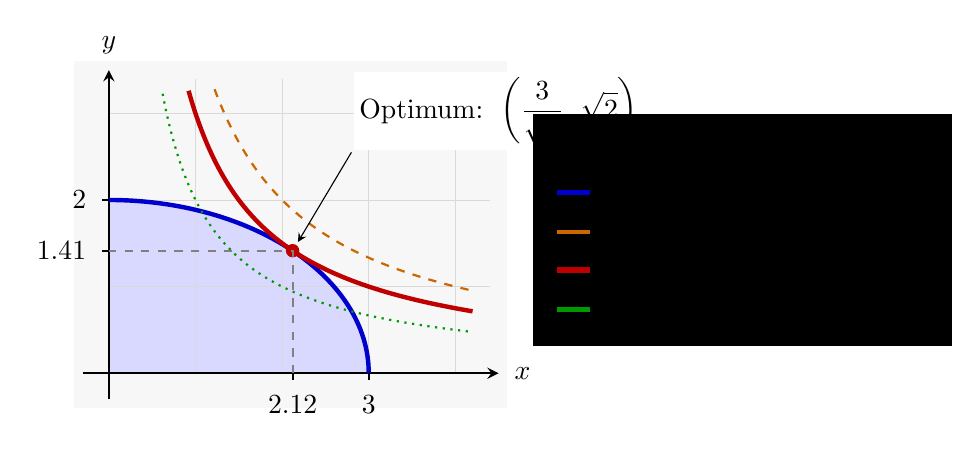
\begin{tikzpicture}[scale=1.1]
    % 1. Background
    \fill[gray!6] (-0.4,-0.4) rectangle (4.6,3.6);
    % Feasible set in first quadrant of 4x^2 + 9y^2 <= 36 -> (x/3)^2 + (y/2)^2 <= 1
    \fill[blue!15] (0,0) -- (3,0) arc[start angle=0, end angle=90, x radius=3, y radius=2] -- cycle;

    % 2. Grid and Axes
    \draw[very thin, gray!30] (0,0) grid (4.4,3.4);
    \draw[->, >=stealth, thick] (-0.3,0) -- (4.5,0) node[right=2pt, black] {$x$};
    \draw[->, >=stealth, thick] (0,-0.3) -- (0,3.5) node[above=2pt, black] {$y$};

    % 3. Primary plots
    % Elliptical constraint boundary: 4x^2 + 9y^2 = 36
    \draw[ultra thick, blue!80!black] (3,0) arc[start angle=0, end angle=90, x radius=3, y radius=2];

    % Hyperbola indifference curves xy = c
    % c = 3 (tangent at (3/sqrt(2), sqrt(2)) = (2.121, 1.414))
    \draw[ultra thick, red!75!black, domain=0.92:4.2, samples=80, smooth] plot (\x, {3/\x});
    % c = 4 (infeasible)
    \draw[thick, dashed, orange!80!black, domain=1.22:4.2, samples=80, smooth] plot (\x, {4/\x});
    % c = 2 (suboptimal)
    \draw[thick, dotted, green!60!black, domain=0.62:4.2, samples=80, smooth] plot (\x, {2/\x});

    % Tangent optimal point
    \fill[red!75!black] (2.1213, 1.4142) circle (2.2pt);

    % Explicit ticks
    \draw[thick] (3,0) -- (3,-0.08) node[below=2pt, black] {$3$};
    \draw[thick] (0,2) -- (-0.08,2) node[left=2pt, black] {$2$};
    \draw[thick, dashed, gray] (2.1213,0) -- (2.1213,1.4142) -- (0,1.4142);
    \draw[thick] (2.1213,0) -- (2.1213,-0.08) node[below=2pt, black] {$2.12$};
    \draw[thick] (0,1.4142) -- (-0.08,1.4142) node[left=2pt, black] {$1.41$};

    % 4. Off-axis callouts and single-node legend
    \draw[->, >=stealth, thin, black, shorten >=2pt] (2.8, 2.55) -- (2.15, 1.46);
    \node[above right=1pt, align=left, black, fill=white, inner sep=2pt] at (2.8, 2.55) {$\displaystyle \text{Optimum: }\left(\frac{3}{\sqrt{2}},\,\sqrt{2}\right)$};

    \node[draw, thick, fill=white, align=left, inner sep=8pt, anchor=west, black] at (4.9, 1.65) {
        \textbf{Ellipsoidal Constraint}\\[4pt]
        \textcolor{blue!80!black}{\rule[0.5ex]{1.2em}{2pt}} Constraint: $4x^2 + 9y^2 = 36$\\[2pt]
        \textcolor{orange!80!black}{\rule[0.5ex]{1.2em}{1.5pt}} Infeasible: $xy = 4$\\[2pt]
        \textcolor{red!75!black}{\rule[0.5ex]{1.2em}{2pt}} Optimal Tangent: $xy = 3$\\[2pt]
        \textcolor{green!60!black}{\rule[0.5ex]{1.2em}{1.5pt}} Suboptimal: $xy = 2$
    };
\end{tikzpicture}
\end{center}

\begin{example}[Ellipsoidal Constraint]
Maximize $Q(x, y) = 2xy$ subject to the elliptical constraint $9x^2 + 16y^2 = 144$.

\textbf{Solution:} Divide the constraint by $144$ to rewrite it in standard unit-sum form:
\[
\left(\frac{x}{4}\right)^2 + \left(\frac{y}{3}\right)^2 = 1.
\]
Define $u_1 = \frac{x}{4}$ and $u_2 = \frac{y}{3}$, so $x = 4u_1$ and $y = 3u_2$. Then $\mathbf{u} = (u_1, u_2)^T$ satisfies $\mathbf{u}^T \mathbf{u} = u_1^2 + u_2^2 = 1$, and the objective function becomes
\[
\tilde{Q}(\mathbf{u}) = 2(4u_1)(3u_2) = 24u_1 u_2 = \mathbf{u}^T \begin{bmatrix} 0 & 12 \\ 12 & 0 \end{bmatrix} \mathbf{u}.
\]
The eigenvalues of $\begin{bmatrix} 0 & 12 \\ 12 & 0 \end{bmatrix}$ are $\lambda_1 = 12$ and $\lambda_2 = -12$, with unit maximizer $\mathbf{u}_1 = \frac{1}{\sqrt{2}}(1, 1)^T$ (or $-\mathbf{u}_1$). By Theorem~6, the maximum value of $Q$ is $12$, attained at
\[
x = 4\left(\frac{1}{\sqrt{2}}\right) = 2\sqrt{2}, \qquad y = 3\left(\frac{1}{\sqrt{2}}\right) = \frac{3}{\sqrt{2}}
\]
(and at $(-2\sqrt{2}, -3/\sqrt{2})$).
\end{example}

\subsection{Constrained Minimization and Sequential Minimization ($\lambda_n, \lambda_{n-1}$)}
The homework exclusively asked for constrained \emph{maxima}. However, Theorem~6 equally states that the constrained \emph{minimum} $m$ on $\mathbf{x}^T \mathbf{x} = 1$ is the least eigenvalue $\lambda_n$, attained at $\mathbf{u}_n$. Analogously, minimizing $\mathbf{x}^T A \mathbf{x}$ subject to $\mathbf{x}^T \mathbf{x} = 1$ and $\mathbf{x}^T \mathbf{u}_n = 0$ yields the second least eigenvalue $\lambda_{n-1}$, attained at $\mathbf{u}_{n-1}$.

\begin{example}[Sequential Constrained Minimization]
Find the minimum value of $Q(\mathbf{x}) = 2x_1^2 + 5x_2^2 + 2x_3^2 + 4x_1x_3$ subject to $\mathbf{x}^T \mathbf{x} = 1$ and $\mathbf{x}^T \mathbf{u}_3 = 0$, where $\mathbf{u}_3$ is a unit eigenvector corresponding to the least eigenvalue $\lambda_3$ of $Q$.

\textbf{Solution:} The symmetric matrix is $A = \begin{bmatrix} 2 & 0 & 2 \\ 0 & 5 & 0 \\ 2 & 0 & 2 \end{bmatrix}$. Its characteristic equation is
\[
(5 - \lambda)\bigl((2-\lambda)^2 - 4\bigr) = (5 - \lambda)\lambda(\lambda - 4) = 0,
\]
so the eigenvalues in descending order are $\lambda_1 = 5 > \lambda_2 = 4 > \lambda_3 = 0$. The least eigenvalue is $\lambda_3 = 0$ (with $\mathbf{u}_3 = \frac{1}{\sqrt{2}}(1, 0, -1)^T$). Under $\mathbf{x} = P\mathbf{y}$, the constraint $\mathbf{x}^T \mathbf{u}_3 = 0$ sets $y_3 = 0$, leaving $y_1^2 + y_2^2 = 1$ and
\[
Q(\mathbf{x}) = 5y_1^2 + 4y_2^2 \ge 4(y_1^2 + y_2^2) = 4.
\]
Hence the constrained minimum is $\lambda_2 = 4$, attained at $\mathbf{u}_2 = \frac{1}{\sqrt{2}}(1, 0, 1)^T$.
\end{example}

\subsection{Generalized Rayleigh Quotients ($\frac{\mathbf{x}^T A \mathbf{x}}{\mathbf{x}^T B \mathbf{x}}$)}
In signal processing (Linear Discriminant Analysis) and structural vibration, one optimizes the ratio $R(\mathbf{x}) = \frac{\mathbf{x}^T A \mathbf{x}}{\mathbf{x}^T B \mathbf{x}}$ for $\mathbf{x} \neq \mathbf{0}$, where $A$ is symmetric and $B$ is symmetric positive definite ($B \succ 0$). Because $R(c\mathbf{x}) = R(\mathbf{x})$ for any $c \neq 0$, this is equivalent to optimizing $\mathbf{x}^T A \mathbf{x}$ subject to the generalized norm constraint $\mathbf{x}^T B \mathbf{x} = 1$. Factoring $B = C^T C$ (via Cholesky or $B^{1/2}$) and substituting $\mathbf{y} = C\mathbf{x}$ transforms the problem into $\max_{\mathbf{y}^T\mathbf{y}=1} \mathbf{y}^T (C^{-T} A C^{-1})\mathbf{y}$.

\begin{example}[Generalized Rayleigh Quotient]
Find the maximum value of $R(\mathbf{x}) = \frac{3x_1^2 + 8x_2^2}{x_1^2 + 4x_2^2}$ over all nonzero $\mathbf{x} \in \R^2$.

\textbf{Solution:} By scale invariance, maximize $3x_1^2 + 8x_2^2$ subject to $x_1^2 + 4x_2^2 = 1$. Set $y_1 = x_1$ and $y_2 = 2x_2$ (so $y_1^2 + y_2^2 = 1$). Then $x_1 = y_1$ and $x_2 = y_2/2$, giving
\[
3x_1^2 + 8x_2^2 = 3y_1^2 + 8\left(\frac{y_2}{2}\right)^2 = 3y_1^2 + 2y_2^2.
\]
By Theorem~6, the maximum over $y_1^2 + y_2^2 = 1$ is $\lambda_1 = 3$ (attained at $\mathbf{y} = (1, 0)^T \implies \mathbf{x} = (1, 0)^T$).
\end{example}

\subsection{Equivalence to Lagrange Multipliers and the Courant–Fischer Min-Max Theorem}
In multivariable calculus, maximizing $Q(\mathbf{x}) = \mathbf{x}^T A \mathbf{x}$ subject to $g(\mathbf{x}) = \mathbf{x}^T \mathbf{x} - 1 = 0$ via Lagrange multipliers sets $\nabla Q(\mathbf{x}) = \lambda \nabla g(\mathbf{x})$. Because $\nabla(\mathbf{x}^T A \mathbf{x}) = 2A\mathbf{x}$ (when $A$ is symmetric) and $\nabla(\mathbf{x}^T \mathbf{x} - 1) = 2\mathbf{x}$, the Lagrange condition becomes
\[
2A\mathbf{x} = \lambda (2\mathbf{x}) \iff A\mathbf{x} = \lambda \mathbf{x},
\]
proving directly from calculus why critical points on the unit sphere must be eigenvectors! Moreover, the \textbf{Courant–Fischer Min-Max Theorem} generalizes Theorem~8 without requiring prior knowledge of $\mathbf{u}_1, \dots, \mathbf{u}_{k-1}$:
\[
\lambda_k = \max_{\dim(W)=k} \; \min_{\substack{\mathbf{x} \in W \\ \|\mathbf{x}\| = 1}} \mathbf{x}^T A \mathbf{x} = \min_{\dim(V)=n-k+1} \; \max_{\substack{\mathbf{x} \in V \\ \|\mathbf{x}\| = 1}} \mathbf{x}^T A \mathbf{x}.
\]

\begin{example}[Bounding an Eigenvalue via Courant–Fischer]
Let $A = \begin{bmatrix} 6 & 2 & 0 \\ 2 & 3 & 0 \\ 0 & 0 & 1 \end{bmatrix}$. Use the Courant–Fischer theorem with the coordinate plane $V = \{\mathbf{x} \in \R^3 : x_1 = 0\}$ to obtain an upper bound on the middle eigenvalue $\lambda_2$ without computing the eigenvalues of $A$.

\textbf{Solution:} Since $\dim(V) = 2 = 3 - 2 + 1$, Courant–Fischer guarantees
\[
\lambda_2 \le \max_{\substack{\mathbf{x} \in V \\ \|\mathbf{x}\| = 1}} \mathbf{x}^T A \mathbf{x}.
\]
For $\mathbf{x} = (0, x_2, x_3)^T \in V$ with $x_2^2 + x_3^2 = 1$, we have $\mathbf{x}^T A \mathbf{x} = 3x_2^2 + x_3^2 \le 3(x_2^2 + x_3^2) = 3$. Thus $\lambda_2 \le 3$ immediately. (Indeed, the exact eigenvalues of $A$ are $7, 2, 1$, so $\lambda_2 = 2 \le 3$.)
\end{example}

% ==============================================================================
% PART 8
% ==============================================================================
\section{Advanced Diagnostic Testing: ``Find the Flaw''}

Each of the five problems below is accompanied by a complete, plausible-looking solution containing a \textbf{single, subtle, yet critical flaw} that produces an incorrect final answer. Your task as a grader is to pinpoint the error, state in one sentence why it is invalid, and supply the corrected step and solution. A full Grader's Diagnostic Key follows in Subsection~\ref{subsec:diagnostic_key}.

\subsection{Diagnostic Problems (Flawed Solutions)}

\begin{example}[Diagnostic Problem 1]
\textbf{Problem:} Find the maximum value of $Q(\mathbf{x}) = 2x_1^2 + 2x_2^2 + 6x_1x_2$ subject to $\mathbf{x}^T \mathbf{x} = 1$.

\textbf{Flawed Solution:}
We write $Q(\mathbf{x}) = \mathbf{x}^T A \mathbf{x}$, where the symmetric matrix of the quadratic form is
\[
A = \begin{bmatrix} 2 & 6 \\ 6 & 2 \end{bmatrix}.
\]
To find the eigenvalues of $A$, we solve the characteristic equation $\det(A - \lambda I) = 0$:
\[
(2 - \lambda)^2 - 36 = 0 \implies 2 - \lambda = \pm 6 \implies \lambda_1 = 8, \quad \lambda_2 = -4.
\]
By Theorem~6, the maximum value of $Q(\mathbf{x})$ subject to $\mathbf{x}^T \mathbf{x} = 1$ is the greatest eigenvalue of $A$. Thus the maximum value is $8$.
\end{example}

\begin{example}[Diagnostic Problem 2]
\textbf{Problem:} Find a unit vector $\mathbf{x} \in \R^2$ at which $Q(\mathbf{x}) = 5x_1^2 + 5x_2^2 + 6x_1x_2$ is maximized subject to $\mathbf{x}^T \mathbf{x} = 1$.

\textbf{Flawed Solution:}
The symmetric matrix of $Q(\mathbf{x})$ is $A = \begin{bmatrix} 5 & 3 \\ 3 & 5 \end{bmatrix}$. Its characteristic equation is $(5 - \lambda)^2 - 9 = 0$, giving eigenvalues $\lambda_1 = 8$ and $\lambda_2 = 2$. Solving $(A - 8I)\mathbf{x} = \mathbf{0}$ and $(A - 2I)\mathbf{x} = \mathbf{0}$ and normalizing yields orthonormal eigenvectors
\[
\mathbf{u}_1 = \begin{bmatrix} 1/\sqrt{2} \\ 1/\sqrt{2} \end{bmatrix}, \qquad \mathbf{u}_2 = \begin{bmatrix} -1/\sqrt{2} \\ 1/\sqrt{2} \end{bmatrix}.
\]
Setting $P = \begin{bmatrix} \mathbf{u}_1 & \mathbf{u}_2 \end{bmatrix}$, the orthogonal change of variable $\mathbf{x} = P\mathbf{y}$ transforms the problem into maximizing $\mathbf{y}^T D \mathbf{y} = 8y_1^2 + 2y_2^2$ subject to $y_1^2 + y_2^2 = 1$. Since $8y_1^2 + 2y_2^2 \le 8(y_1^2 + y_2^2) = 8$, equality is achieved at $\mathbf{e}_1 = \begin{bmatrix} 1 \\ 0 \end{bmatrix}$. Therefore, $Q(\mathbf{x})$ is maximized at the unit vector $\mathbf{x} = \begin{bmatrix} 1 \\ 0 \end{bmatrix}$.
\end{example}

\begin{example}[Diagnostic Problem 3]
\textbf{Problem:} Find the maximum value of $Q(\mathbf{x}) = -7x_1^2 + x_2^2 + 6x_1x_2$ subject to $\mathbf{x}^T \mathbf{x} = 1$.

\textbf{Flawed Solution:}
The symmetric matrix representing $Q(\mathbf{x})$ is $A = \begin{bmatrix} -7 & 3 \\ 3 & 1 \end{bmatrix}$. Its characteristic equation is
\[
(-7 - \lambda)(1 - \lambda) - 9 = \lambda^2 + 6\lambda - 16 = (\lambda + 8)(\lambda - 2) = 0,
\]
so the eigenvalues of $A$ are $-8$ and $2$. Because $|-8| = 8 > |2| = 2$, the dominant eigenvalue of $A$ (with greatest magnitude) is $-8$. By Theorem~6, the maximum value of $Q(\mathbf{x})$ on the unit circle is $-8$ (or magnitude $8$).
\end{example}

\begin{example}[Diagnostic Problem 4]
\textbf{Problem:} Find the maximum value of $Q(\mathbf{x}) = 4x_1 x_2$ subject to the constraint $x_1^2 + 4x_2^2 = 1$.

\textbf{Flawed Solution:}
We express $Q(\mathbf{x})$ in matrix form $Q(\mathbf{x}) = \mathbf{x}^T A \mathbf{x}$, where
\[
A = \begin{bmatrix} 0 & 2 \\ 2 & 0 \end{bmatrix}.
\]
The characteristic equation of $A$ is $\lambda^2 - 4 = 0$, giving eigenvalues $\lambda_1 = 2$ and $\lambda_2 = -2$. By Theorem~6, the constrained maximum value of $Q(\mathbf{x})$ is the greatest eigenvalue of $A$, which is $2$.
\end{example}

\begin{example}[Diagnostic Problem 5]
\textbf{Problem:} Let $Q(\mathbf{x}) = 6x_1^2 + 3x_2^2 + x_3^2$. Find the maximum value of $Q(\mathbf{x})$ subject to the constraints $\mathbf{x}^T \mathbf{x} = 1$ and $\mathbf{x}^T \mathbf{w} = 0$, where $\mathbf{w} = (0, 1, 0)^T$.

\textbf{Flawed Solution:}
The matrix of $Q(\mathbf{x})$ is $A = \operatorname{diag}(6, 3, 1)$, whose eigenvalues in descending order are $\lambda_1 = 6$, $\lambda_2 = 3$, and $\lambda_3 = 1$. Note that $\mathbf{w} = (0, 1, 0)^T$ is a unit eigenvector of $A$. By Theorem~7, the maximum value of $\mathbf{x}^T A \mathbf{x}$ subject to the unit-vector constraint $\mathbf{x}^T \mathbf{x} = 1$ and the orthogonality constraint $\mathbf{x}^T \mathbf{w} = 0$ is the second greatest eigenvalue of $A$, which is $\lambda_2 = 3$.
\end{example}

\subsection{Diagnostic Solutions and Error Analysis Key}
\label{subsec:diagnostic_key}

\begin{enumerate}[label=\textbf{Key \arabic*:}]
    \item \textbf{Error:} In the construction of $A$, the off-diagonal entries were set to $6$ instead of $3$.\\
    \textbf{Why It Is an Error:} The coefficient of a cross-product term $c_{12} x_1 x_2$ must be split equally between $a_{12}$ and $a_{21}$ ($a_{12} = a_{21} = c_{12}/2$) so that $\mathbf{x}^T A \mathbf{x}$ equals $Q(\mathbf{x})$ rather than doubling the cross term.\\
    \textbf{Corrected Step and Final Solution:} The true matrix is $A = \begin{bmatrix} 2 & 3 \\ 3 & 2 \end{bmatrix}$, with characteristic equation $(2-\lambda)^2 - 9 = 0 \implies \lambda = 5, -1$. The correct maximum value is $5$.

    \item \textbf{Error:} The solution concluded that $\mathbf{x} = \mathbf{e}_1 = (1, 0)^T$ maximizes $Q(\mathbf{x})$.\\
    \textbf{Why It Is an Error:} The vector $\mathbf{y} = \mathbf{e}_1$ maximizes the diagonalized form $\mathbf{y}^T D \mathbf{y}$ in $\mathbf{y}$-coordinates, so one must map it back to $\mathbf{x}$-coordinates using $\mathbf{x} = P\mathbf{e}_1 = \mathbf{u}_1$.\\
    \textbf{Corrected Step and Final Solution:} Computing $\mathbf{x} = P\mathbf{e}_1 = \mathbf{u}_1$ yields the true unit maximizer $\mathbf{x} = \begin{bmatrix} 1/\sqrt{2} \\ 1/\sqrt{2} \end{bmatrix}$ (where $Q(\mathbf{x}) = 8$, whereas $Q(1,0) = 5$).

    \item \textbf{Error:} The solution chose $\lambda = -8$ as the maximum because $|-8| > |2|$.\\
    \textbf{Why It Is an Error:} In Theorem~6, \emph{greatest} and \emph{least} eigenvalues refer strictly to the natural ordering of real numbers ($\lambda_1 \ge \lambda_n$), not to absolute magnitudes.\\
    \textbf{Corrected Step and Final Solution:} Ordering the eigenvalues on $\R$ gives $2 > -8$, so $\lambda_1 = 2$ is the constrained maximum (and $-8$ is the constrained minimum). The correct maximum value is $2$.

    \item \textbf{Error:} The solution applied Theorem~6 directly to $A = \begin{bmatrix} 0 & 2 \\ 2 & 0 \end{bmatrix}$ without converting the elliptical constraint $x_1^2 + 4x_2^2 = 1$ to a unit-sphere constraint.\\
    \textbf{Why It Is an Error:} Theorem~6 only applies when the constraint is the Euclidean unit sphere $\mathbf{x}^T \mathbf{x} = 1$, whereas $x_1^2 + 4x_2^2 = 1$ allows $|x_2|$ to be at most $1/2$ rather than $1$.\\
    \textbf{Corrected Step and Final Solution:} Set $u_1 = x_1$ and $u_2 = 2x_2$, so $u_1^2 + u_2^2 = 1$ and $Q = 4 u_1 (u_2 / 2) = 2 u_1 u_2 = \mathbf{u}^T \begin{bmatrix} 0 & 1 \\ 1 & 0 \end{bmatrix}\mathbf{u}$. The eigenvalues of the rescaled matrix are $\pm 1$, so the correct maximum value is $1$.

    \item \textbf{Error:} The solution invoked Theorem~7 despite $\mathbf{w} = (0, 1, 0)^T$ being an eigenvector for $\lambda_2 = 3$ rather than $\lambda_1 = 6$.\\
    \textbf{Why It Is an Error:} Theorem~7 applies exclusively when the orthogonality constraint $\mathbf{x}^T \mathbf{u}_1 = 0$ removes the eigenspace of the \emph{greatest} eigenvalue $\lambda_1$, not an intermediate eigenvalue.\\
    \textbf{Corrected Step and Final Solution:} The constraint $\mathbf{x}^T \mathbf{w} = 0$ simply sets $x_2 = 0$, leaving $Q(\mathbf{x}) = 6x_1^2 + x_3^2$ subject to $x_1^2 + x_3^2 = 1$. Since $6x_1^2 + x_3^2 \le 6(x_1^2 + x_3^2) = 6$ with equality at $\mathbf{x} = (1, 0, 0)^T$, the correct maximum value is $6$.
\end{enumerate}

\end{document}